\part{12/2}

\section{Abstand eines Punktes von einer Geraden}
gegeben:
\begin{gather*}
  g \colon \vv{x} = \vv{a} + r \cdot \vv{b} \\
  P: \vv{p}
\end{gather*}
\begin{gather*}
  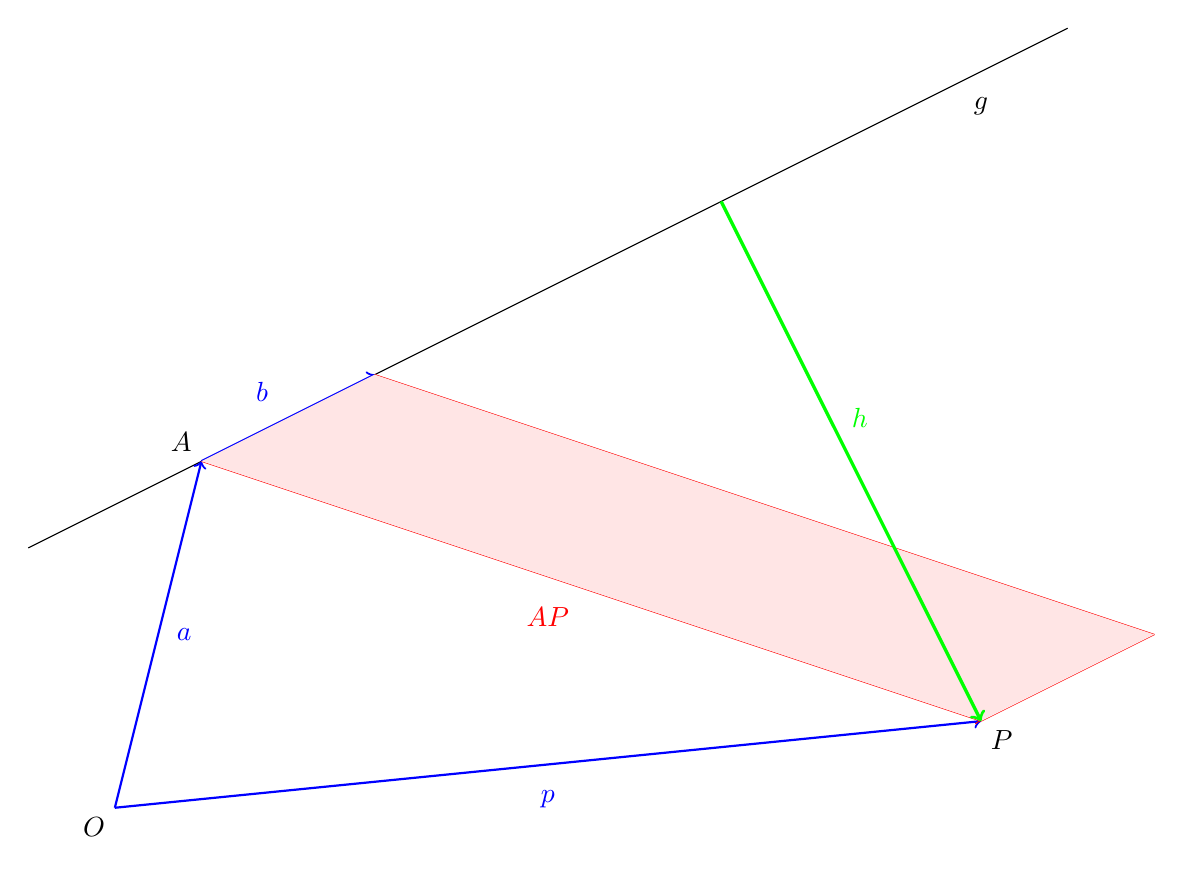
\begin{tikzpicture}[scale=1.1]
    \coordinate (O) at (0,0);
    \coordinate (A) at (1,4);
    \coordinate (B) at (3,5);
    \coordinate (P) at (10,1);
    \coordinate (Q) at (12,2);
    \draw (-1,3) -- (11,9);
    \draw[->,blue,thick] (O) -- (A);
    \draw[->,blue,thick] (O) -- (P);
    \draw[->,blue,thick] (A) -- (B);
    \draw[->,red] (A) -- (P);
    \draw[red] (B) -- (Q);
    \draw[red] (P) -- (Q);
    \fill[red!10] (A) -- (B) -- (Q) -- (P) -- cycle;
    \draw[->,green,very thick] (7,7) -- (P);
    \node[below left] at (O) {$O$};
    \node[above left] at (A) {$A$};
    \node[below right] at (P) {$P$};
    \node at (10,8.1) {$g$};
    \node[blue] at (0.8,2) {$\vv{a}$};
    \node[blue] at (1.7,4.8) {$\vv{b}$};
    \node[blue] at (5,0.1) {$\vv{p}$};
    \node[green] at (8.6,4.5) {$\vv{h}$};
    \node[red] at (5,2.2) {$\vv{AP}$};
  \end{tikzpicture}
\end{gather*}
\begin{gather*}
  \text{Bilde } |\vv{b} \times \vv{AP}| = A_{Parallelogramm} \\
  |\vv{b}| \cdot |\vv{h}| = A_{Parallelogramm} \\\\
  |\vv{b} \times \vv{AP}| = |\vv{b}| \cdot |\vv{h}| \\
  \;\Rightarrow\quad \frac{|\vv{b} \times \vv{AP}|}{|\vv{b}|} = |\vv{h}|
\end{gather*}
$|\vv{h}|$ ist der gesuchte Abstand von Punkt $P$ zur Geraden $g$.
\begin{exercise}{373/5}
  \item [c]
  \begin{gather*}
    g \colon \vv{x} = \begin{pmatrix}1 \\ 1 \\ 0\end{pmatrix} + t \cdot \begin{pmatrix}2 \\ 1 \\ -1\end{pmatrix} \qquad R(-2|-1|1) \\
    \vv{PR} = \begin{pmatrix}-3 \\ -2 \\ 1\end{pmatrix} \qquad \vv{u} = \begin{pmatrix}2 \\ 1 \\ -1\end{pmatrix} \\
    |\vv{h}| = \frac{|\vv{u} \times \vv{PR}|}{|\vv{u}|} = \frac{\left|\begin{pmatrix}-1 \\ 1 \\ -1\end{pmatrix}\right|}{\left|\begin{pmatrix}2 \\ 1 \\ -1\end{pmatrix}\right|} = \frac{\sqrt{3}}{\sqrt{6}} = \sqrt{\frac{1}{2}} \approx 0.7071
  \end{gather*}
  \begin{gather*}
    g \colon \vv{x} = \begin{pmatrix}2 \\ 3 \\ 2\end{pmatrix} + t \cdot \begin{pmatrix}2 \\ -3 \\ -6\end{pmatrix} \qquad R(1|2|-3) \\
    \vv{PR} = \begin{pmatrix}-1 \\ -1 \\ -5\end{pmatrix} \qquad \vv{u} = \begin{pmatrix}2 \\ -3 \\ -6\end{pmatrix} \\
    |\vv{h}| = \frac{|\vv{u} \times \vv{PR}|}{|\vv{u}|} = \frac{\left|\begin{pmatrix}-9 \\ -16 \\ -5\end{pmatrix}\right|}{\left|\begin{pmatrix}2 \\ -3 \\ -6\end{pmatrix}\right|} = \frac{\sqrt{362}}{\sqrt{49}} \approx 2.7180
  \end{gather*}
\end{exercise}
\section{Ebenendarstellung}
\subsection{Normalenform}
\begin{gather*}
  E \colon \vv{x} = \vv{a} + r \cdot \vv{b} + s \cdot \vv{c} \\\\
  E \colon (\vv{x} - \vv{a}) \cdot \vv{n} = 0 \\
  \; \vv{AX} \cdot \vv{n} = 0
\end{gather*}
$\vv{n}$ ... Normalenvektor der Ebene \\
$\vv{a}$ ... Stützvektor, Ortsvektor eines bestimmten Punktes \\
$\vv{x}$ ... allgemeiner Ortsvektor aller Punkte der Ebene \\
$\vv{AX}$ ... Verbindungsvektor, der in der Ebene liegt \\\\
Punkte $X$ der Ebene sind diejenigen, deren Verbindungsvektoren $\vv{AX}$ orthogonal zu $\vv{h}$ stehen. \\\\
z. B.
\begin{gather*}
  \left(\vv{x} - \begin{pmatrix}1 \\ 2 \\ 3\end{pmatrix}\right) \cdot \begin{pmatrix}-1 \\ 0 \\ 4\end{pmatrix} = 0 \\\\
  \text{Beispiellösung } x_1 = \begin{pmatrix}5 \\ 0 \\ 4\end{pmatrix} \\\\
  \text{Punktprobe } P(2|1|1) \quad P \in E ? \\
  \begin{pmatrix}2 - 1 \\ 1 - 2 \\ 1 - 3\end{pmatrix} \cdot \begin{pmatrix}-1 \\ 0 \\ 4\end{pmatrix} = 0 \qquad -1 + 0 - 8 = -9 \neq 0 \quad\Rightarrow\quad P \not\in E
\end{gather*}
Normalengleichung aus $A(1|0|5)$, $B(0|2|1)$, $C(4|5|6)$
\begin{gather*}
  E \colon \vv{x} = \begin{pmatrix}1 \\ 0 \\ 5\end{pmatrix} + r \cdot \begin{pmatrix}-1 \\ 2 \\ -4\end{pmatrix} + s \cdot \begin{pmatrix}3 \\ 5 \\ 1\end{pmatrix} \\
  \vv{n} = \vv{AB} \times \vv{AC} = \begin{pmatrix}-1 \\ 2 \\ -4\end{pmatrix} \times \begin{pmatrix}3 \\ 5 \\ 1\end{pmatrix} = \begin{pmatrix}22 \\ -11 \\ -11\end{pmatrix} \\
  E \colon \left(\vv{x} - \begin{pmatrix}1 \\ 0 \\ 5\end{pmatrix}  \right) \cdot \begin{pmatrix}22 \\ -11 \\ -11\end{pmatrix} = 0
\end{gather*}
\subsection{Koordinatenform}
Berechne das Skalarprodukt in der Normalengleichung mit $\vv{x} = \begin{pmatrix}x_1 \\ x_2 \\ x_3\end{pmatrix}$
\begin{gather*}
  E \colon \left(\begin{pmatrix}x_1 \\ x_2 \\ x_3\end{pmatrix} - \begin{pmatrix}a_1 \\ a_2 \\ a_3\end{pmatrix}\right) \cdot \begin{pmatrix}n_1 \\ n_2 \\ n_3\end{pmatrix} = 0 \\
  \begin{pmatrix}x_1 \\ x_2 \\ x_3\end{pmatrix} \cdot \begin{pmatrix}n_1 \\ n_2 \\ n_3\end{pmatrix} - \begin{pmatrix}a_1 \\ a_2 \\ a_3\end{pmatrix} \cdot \begin{pmatrix}n_1 \\ n_2 \\ n_3\end{pmatrix} = 0 \\
  (n_1 \cdot x_1 + n_2 \cdot x_2 + n_3 \cdot x_3) - (a_1 \cdot n_1 + a_2 \cdot n_2 + a_3 \cdot n_3) = 0 \\\\
  \text{z. B. } 22x_1 - 11x_2 - 11x_3 = -33 \\
  \text{Beispiellösungen } \vv{x} = \begin{pmatrix}-1 \\ 1 \\ 0\end{pmatrix}, \begin{pmatrix}1 \\ 2 \\ 3\end{pmatrix}, \begin{pmatrix}2 \\ 1 \\ 6\end{pmatrix}, ...
\end{gather*}
\begin{gather*}
  E \colon ax_1 + bx_2 + cx_3 = d
\end{gather*}
Betrache die Koordinatenform als eine Gleichung für drei Variablen $x_1$, $x_2$, $x_3$. Die Lösungen der Gleichung sind Dreiertupel $L = \{(...,\;...,\;...),\;...\}$. Notiere ich die Dreiertupel als Spaltenvektoren, so stellen sie die Ortsvektoren der Punkte der Ebene $E$ dar. Die Koeffizienten $a$, $b$, $c$ der Koordinatenform sind die Koordinaten von $\vv{n}$, des Normalenvektors.
\subsubsection{Koordinatenform $\rightarrow$ Normalenform}
\begin{gather*}
  \text{z. B. } 5x_1 - x_2 + 3x_3 = 9
\end{gather*}
\begin{enumerate}
  \item Lies ab $\vv{n} = \begin{pmatrix}5 \\ -1 \\ 3\end{pmatrix}$
  \item Finde eine Lösung $\begin{pmatrix}x_1 \\ x_2 \\ x_3\end{pmatrix}$, z. B. $\begin{pmatrix}0 \\ 0 \\ 3\end{pmatrix}$
\end{enumerate}
\begin{gather*}
  E \colon \left(\vv{x} - \begin{pmatrix}0 \\ 0 \\ 3\end{pmatrix}\right) \cdot \begin{pmatrix}5 \\ -1 \\ 3\end{pmatrix} = 0
\end{gather*}
\subsubsection{Sonderfälle}
\begin{itemize}
  \item
  \begin{gather*}
    E \colon x_3 = 5 \quad\rightarrow\quad \vv{n} = \begin{pmatrix}0 \\ 0 \\ 1\end{pmatrix}
  \end{gather*}
  Punkte der Ebene haben $x_3 = 5$; $x_1$, $x_2$ sind beliebige Koordinaten.
  \begin{gather*}
    \text{z. B. } \begin{pmatrix}1 \\ 1 \\ 5\end{pmatrix}, \begin{pmatrix}-2 \\ 3 \\ 5\end{pmatrix}, \begin{pmatrix}0 \\ 7 \\ 5\end{pmatrix}, ...
  \end{gather*}
  $x_1$ und $x_2$ sind nicht erwähnt, also frei wählbar.
  \item
  \begin{gather*}
    E \colon 2x_1 - 4x_2 = 0
  \end{gather*}
  Der Ursprung $O$ ist Teil der Ebene $E$. Der Verbindungsvektor $\vv{O} - \vv{a}$, also der Ortsvektor $\vv{a}$ liegt in der Ebene $E$ und steht orthogonal zu $\vv{n}$. Daher sind $\vv{a} \cdot \vv{n} = 0$ und damit $d = 0$.
\end{itemize}
\begin{exercise}{325/3}
  \begin{gather*}
    D(-7|1|3)
  \end{gather*}
  \item [a]
  \begin{gather*}
    A(1|1|1) \qquad B(1|0|1) \qquad C(0|1|1) \\
    \vv{AB} = \begin{pmatrix}0 \\ -1 \\ 0\end{pmatrix} \qquad \vv{AC} = \begin{pmatrix}-1 \\ 0 \\ 0\end{pmatrix} \\
    \vv{n} = \vv{AB} \times \vv{AC} = \begin{pmatrix}0 \\ 0 \\ -1\end{pmatrix} \\\\
    E \colon \left(\vv{x} - \begin{pmatrix}1 \\ 1 \\ 1\end{pmatrix}\right) \cdot \begin{pmatrix}0 \\ 0 \\ -1\end{pmatrix} = 0 \\
    E \colon -x_3 = 0 + 0 - 1 = -1 \\\\
    D \in E ? \qquad -x_3 = -3 \neq -1 \qquad \Rightarrow\quad D \not\in E
  \end{gather*}
  \item [b]
  \begin{gather*}
    A(-1|2|0) \qquad B(-3|1|1) \qquad C(1|-1|-1) \\
    \vv{AB} = \begin{pmatrix}-2 \\ -1 \\ 1\end{pmatrix} \qquad \vv{AC} = \begin{pmatrix}2 \\ -3 \\ -1\end{pmatrix} \\
    \vv{n} = \vv{AB} \times \vv{AC} = \begin{pmatrix}4 \\ 0 \\ 8\end{pmatrix} \\\\
    E \colon \left(\vv{x} - \begin{pmatrix}-1 \\ 2 \\ 0\end{pmatrix}\right) \cdot \begin{pmatrix}4 \\ 0 \\ 8\end{pmatrix} = 0 \\
    E \colon 4x_1 + 8x_3 = -4 + 0 + 0 = -4 \\\\
    D \in E? \qquad 4x_1 + 8x_3 = -28 + 24 = -4 \qquad \Rightarrow\quad D \in E
  \end{gather*}
\end{exercise}
\subsection{Ebenen zeichnen}
Zeichne Ebene $E \colon 2x_1 - 3x_2 + 5x_3 = 12$ \\\\
Schnitt mit der ...
\begin{itemize}
  \item [] $x_1$-Achse:
  \begin{gather*}
    x_2 = x_3 = 0 \quad\Rightarrow\quad 2x_1 = 12 \quad x_1 = 6 \quad P(6|0|0)
  \end{gather*}
  \item [] $x_2$-Achse:
  \begin{gather*}
    x_1 = x_3 = 0 \quad\Rightarrow\quad -3x_2 = 12 \quad x_2 = -4 \quad Q(0|-4|0)
  \end{gather*}
  \item [] $x_3$-Achse:
  \begin{gather*}
    x_1 = x_2 = 0 \quad\Rightarrow\quad 5x_3 = 12 \quad x_3 = 2.4 \quad R(0|0|2.4)
  \end{gather*}
\end{itemize}
$P$, $Q$, $R$ heißen Spurpunkte. \\
Gerade durch $P$ und $Q$ (bzw. $Q$ und $R$, $P$ und $R$) heißt Spurgerade.
\begin{gather*}
  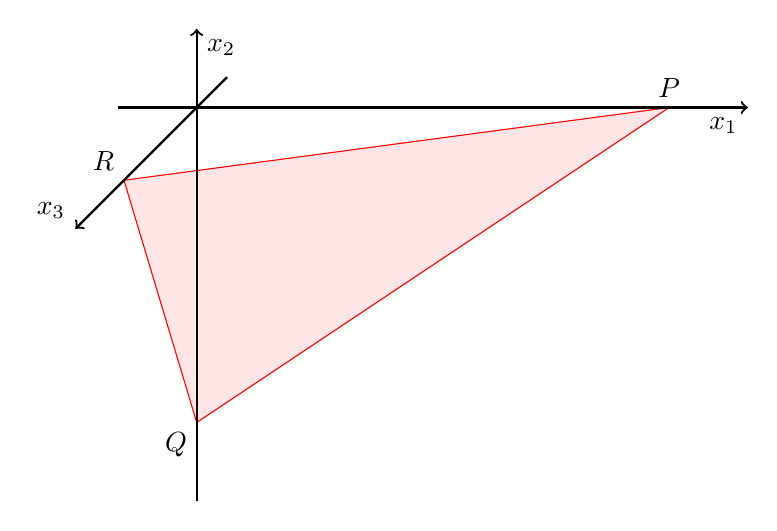
\begin{tikzpicture}
    \coordinate (P) at (6,0,0);
    \coordinate (Q) at (0,-4,0);
    \coordinate (R) at (0,0,2.4);
    \node[above] at (P) {$P$};
    \node[below left] at (Q) {$Q$};
    \node[above left] at (R) {$R$};
    \draw[red,fill=red!10] (P) -- (Q) -- (R) -- (P);
    \draw[thick,->] (-1,0,0) -- (7,0,0) node[anchor=north east]{$x_1$};
    \draw[thick,->] (0,-5,0) -- (0,1,0) node[anchor=north west]{$x_2$};
    \draw[thick,->] (0,0,-1) -- (0,0,4) node[anchor=south east]{$x_3$};
  \end{tikzpicture}
\end{gather*}
Spurgerade (PQ):
\begin{gather*}
  g \colon \vv{x} = \begin{pmatrix}0 \\ -4 \\ 0\end{pmatrix} + r \cdot \begin{pmatrix}6 \\ 4 \\ 0\end{pmatrix}
\end{gather*}
Spezialfälle
\begin{itemize}
  \item
  \begin{gather*}
    3x_1 + 6x_3 = 18 \qquad P(6|0|0) \quad R(0|0|3) \quad Q(0|\infty|0)
  \end{gather*}
  Kein Schnitt mit der $x_2$-Achse, verläuft parallel zur $x_2$-Achse.
  \item
  \begin{gather*}
    2x_1 = 5 \qquad P(2.5|0|0)
  \end{gather*}
  Kein Schnitt mit der $x_2$- und $x_3$-Achse, verläuft parallel zur $x_2x_3$-Ebene.
\end{itemize}
\begin{exercise}{328/3}
  Fig. 1
  \begin{gather*}
    P(2|0|0) \qquad Q(0|5|0) \qquad R(0|0|3) \\
    15x_1 = 30 \qquad 6x_2 = 30 \qquad 10x_3 = 30 \\
    E \colon 15x_1 + 6x_2 + 10x_3 = 30
  \end{gather*}
  Fig. 2
  \begin{gather*}
    P(1|0|0) \qquad Q(0|4|0) \qquad R(0|0|-1.5) \\
    12x_1 = 12 \qquad 3x_2 = 12 \qquad -8x_3 = 12 \\
    E \colon 12x_1 + 3x_2 - 8x_3 = 12
  \end{gather*}
\end{exercise}
\begin{exercise}{328/5}
  \item [a]
  \begin{gather*}
    E \colon \vv{x} = \begin{pmatrix}1 \\ 2 \\ 3\end{pmatrix} + r \cdot \begin{pmatrix}-1 \\ 2 \\ 0\end{pmatrix} + s \cdot \begin{pmatrix}1 \\ 0 \\ 3\end{pmatrix} \\
    \vv{n} = \begin{pmatrix}-1 \\ 2 \\ 0\end{pmatrix} \times \begin{pmatrix}1 \\ 0 \\ 3\end{pmatrix} = \begin{pmatrix}6 \\ 3 \\ -2\end{pmatrix} \qquad \begin{pmatrix}1 \\ 2 \\ 3\end{pmatrix} \cdot \vv{n} = 6 \\
    E \colon 6x_1 + 3x_2 - 2x_3 = 6 \\
    P(1|0|0) \qquad Q(0|2|0) \qquad R(0|0|-3)
  \end{gather*}
  \begin{gather*}
    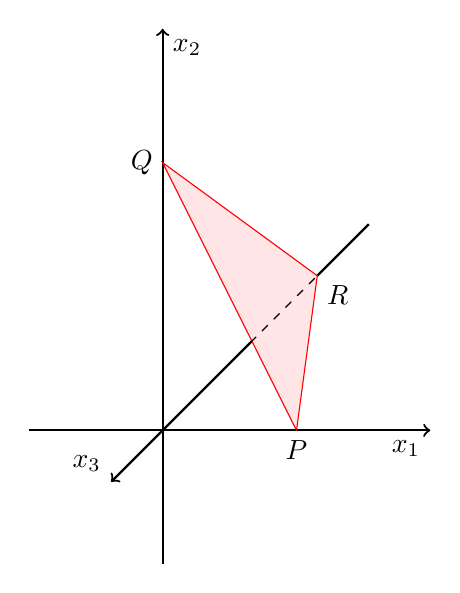
\begin{tikzpicture}[scale=1.7]
      \coordinate (P) at (1,0,0);
      \coordinate (Q) at (0,2,0);
      \coordinate (R) at (0,0,-3);
      \node[below] at (P) {$P$};
      \node[left] at (Q) {$Q$};
      \node[below right] at (R) {$R$};
      \draw[thick,->] (-1,0,0) -- (2,0,0) node[anchor=north east]{$x_1$};
      \draw[thick,->] (0,-1,0) -- (0,3,0) node[anchor=north west]{$x_2$};
      \draw[thick,->] (0,0,-4) -- (0,0,1) node[anchor=south east]{$x_3$};
      \draw[red,fill=red!10] (P) -- (Q) -- (R) -- (P);
      \draw[dashed] (0,0,-1.7) -- (R);
    \end{tikzpicture}
  \end{gather*}
  \item [b]
  \begin{gather*}
    E \colon \vv{x} = \begin{pmatrix}1 \\ 1 \\ 1\end{pmatrix} + r \cdot \begin{pmatrix}5 \\ 0 \\ 5\end{pmatrix} + s \cdot \begin{pmatrix}0 \\ 1 \\ 4\end{pmatrix} \\
    \vv{n} = \begin{pmatrix}5 \\ 0 \\ 5\end{pmatrix} \times \begin{pmatrix}0 \\ 1 \\ 4\end{pmatrix} = \begin{pmatrix}-5 \\ -20 \\ 5\end{pmatrix} \qquad \begin{pmatrix}1 \\ 1 \\ 1\end{pmatrix} \cdot \vv{n} = -20 \\
    E \colon -5x_1 - 20x_2 + 5x_3 = -20 \\
    P(4|0|0) \qquad Q(0|1|0) \qquad R(0|0|-4)
  \end{gather*}
  \begin{gather*}
    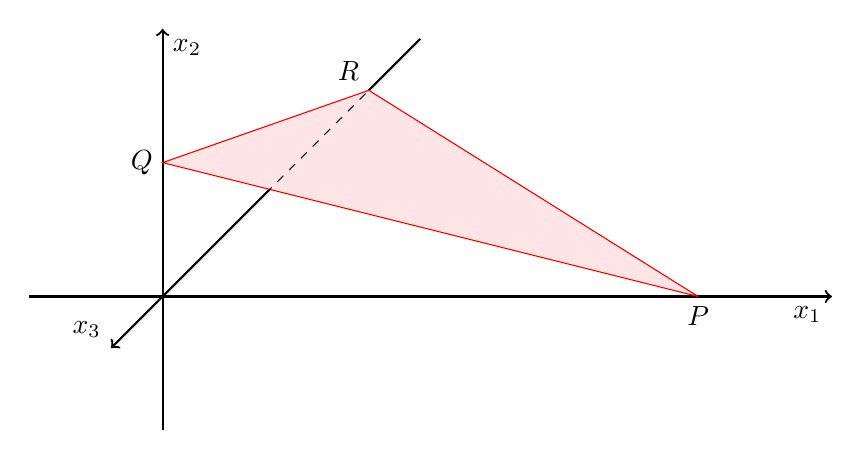
\begin{tikzpicture}[scale=1.7]
      \coordinate (P) at (4,0,0);
      \coordinate (Q) at (0,1,0);
      \coordinate (R) at (0,0,-4);
      \node[below] at (P) {$P$};
      \node[left] at (Q) {$Q$};
      \node[above left] at (R) {$R$};
      \draw[thick,->] (-1,0,0) -- (5,0,0) node[anchor=north east]{$x_1$};
      \draw[thick,->] (0,-1,0) -- (0,2,0) node[anchor=north west]{$x_2$};
      \draw[thick,->] (0,0,-5) -- (0,0,1) node[anchor=south east]{$x_3$};
      \draw[red,fill=red!10] (P) -- (Q) -- (R) -- (P);
      \draw[dashed] (0,0,-2) -- (R);
    \end{tikzpicture}
  \end{gather*}
\end{exercise}
\begin{exercise}{328/6}
  Fig. 3
  \begin{gather*}
    P(0|3|0) \\
    E \colon x_2 = 3 \\
    \text{parallel zur $x_1x_3$-Ebene}
  \end{gather*}
  Fig. 4
  \begin{gather*}
    P(1|0|0) \qquad Q(0|5|0) \\
    5x_1 = 5 \qquad x_2 = 5 \\
    E \colon 5x_1 + x_2 = 5 \\
    \text{parallel zur $x_3$-Ebene}
  \end{gather*}
\end{exercise}
\section{Lage Ebene $\leftrightarrow$ Gerade}
\begin{itemize}
  \item schneiden sich
  \item verlaufen parallel
  \item Gerade ist Teil der Ebene
\end{itemize}
Beispiel:
\begin{gather*}
  E \colon 2x_1 - x_2 + 3x_3 = 16 \\
  g \colon \vv{x} = \begin{pmatrix}1 \\ 2 \\ 3\end{pmatrix} + r \cdot \begin{pmatrix}2 \\ -1 \\ 0\end{pmatrix} = \begin{pmatrix}1 + 2r \\ 2 - r \\ 3\end{pmatrix} = \begin{pmatrix}x_1 \\ x_2 \\ x_3\end{pmatrix} \\\\
  \text{$g$ in $E$ eingesetzt} \\
  2 \cdot (1 + 2r) - (2 - r) + 3 \cdot 3 = 16 \\
  \Rightarrow\quad r = \frac{7}{5} \\
  \text{Schnittpunkt } \vv{OS} = \begin{pmatrix}1 \\ 2 \\ 3\end{pmatrix} + \frac{7}{5} \cdot \begin{pmatrix}2 \\ -1 \\ 0\end{pmatrix} = \begin{pmatrix}3.8 \\ 0.6 \\ 3\end{pmatrix}
\end{gather*}
\begin{itemize}
  \item eindeutige Lösung für $r$ $\Rightarrow$ schneiden sich
  \item kein $r$ erfüllt die Gleichung $\Rightarrow$ kein Schnittpunkt, parallele Lage
  \item für jedes $r$ ein möglicher gemeinsamer Punkt $\Rightarrow$ Gerade liegt in der Ebene
\end{itemize}
\begin{exercise}{330/1}
  \begin{gather*}
    g \colon \vv{x} = \begin{pmatrix}4 \\ 6 \\ 2\end{pmatrix} + t \cdot \begin{pmatrix}1 \\ 2 \\ 3\end{pmatrix}
  \end{gather*}
  \item [a]
  \begin{gather*}
    E \colon 2x_1 + 4x_2 + 6x_3 = 16 \\\\
    2 \cdot (4 + t) + 4 \cdot (6 + 2t) + 6 \cdot (2 + 3t) = 16 \\
    \Rightarrow\quad t = -1 \\\\
    \begin{pmatrix}4 \\ 6 \\ 2\end{pmatrix} - 1 \cdot \begin{pmatrix}1 \\ 2 \\ 3\end{pmatrix} = \begin{pmatrix}3 \\ 4 \\ -1\end{pmatrix} \\\\
    S(3|4|-1)
  \end{gather*}
  \item [b]
  \begin{gather*}
    E \colon 5x_2 - 7x_3 = 13 \\\\
    5 \cdot (6 + 2t) - 7 \cdot (2 + 3t) = 13 \\
    t = \frac{3}{11} \\\\
    \begin{pmatrix}4 \\ 6 \\ 2\end{pmatrix} + \frac{3}{11} \cdot \begin{pmatrix}1 \\ 2 \\ 3\end{pmatrix} = \begin{pmatrix}4.\overline{27} \\ 6.\overline{54} \\ 2.\overline{81}\end{pmatrix} \\\\
    S(4.\overline{27}|6.\overline{54}|2.\overline{81})
  \end{gather*}
\end{exercise}
\begin{exercise}{330/2}
  \item [a]
  \begin{gather*}
    g \colon \vv{x} = \begin{pmatrix}-2 \\ 1 \\ 4\end{pmatrix} + t \cdot \begin{pmatrix}7 \\ 8 \\ 6\end{pmatrix} \qquad E \colon \vv{x} = \begin{pmatrix}1 \\ 4 \\ 3\end{pmatrix} + r \cdot \begin{pmatrix}0 \\ -1 \\ 1\end{pmatrix} + s \cdot \begin{pmatrix}1 \\ 0 \\ 3\end{pmatrix} \\\\
    -2 + 7t = 1 + s \\
    1 + 8t = 4 - r \\
    4 + 6t = 3 + r + 3s \\
    t = 1 \qquad r = -5 \qquad s = 4 \\\\
    \begin{pmatrix}-2 \\ 1 \\ 4\end{pmatrix} + 1 \cdot \begin{pmatrix}7 \\ 8 \\ 6\end{pmatrix} = \begin{pmatrix}5 \\ 9 \\ 10\end{pmatrix} \\\\
    S(5|9|10)
  \end{gather*}
  \item [b]
  \begin{gather*}
    g \colon \vv{x} = \begin{pmatrix}22 \\ -18 \\ -7\end{pmatrix} + t \cdot \begin{pmatrix}4 \\ 1 \\ -5\end{pmatrix} \qquad E \colon \vv{x} = \begin{pmatrix}2 \\ 1 \\ 0\end{pmatrix} + r \cdot \begin{pmatrix}4 \\ -7 \\ 1\end{pmatrix} + s \cdot \begin{pmatrix}0 \\ 4 \\ -3\end{pmatrix} \\\\
    22 + 4t = 2 + 4r \\
    -18 + t = 1 - 7r + 4s \\
    -7 - 5t = r - 3s \\\\
    t = r - 5 \qquad s = 2r - 6 \\\\
    g \in E
  \end{gather*}
  \item [c]
  \begin{gather*}
    g \colon \vv{x} = t \cdot \begin{pmatrix}-1 \\ -1 \\ -1\end{pmatrix} \qquad E \colon \vv{x} = \begin{pmatrix}0 \\ 0 \\ 2\end{pmatrix} + r \cdot \begin{pmatrix}2 \\ 0 \\ 0\end{pmatrix} + s \cdot \begin{pmatrix}0 \\ 2 \\ 0\end{pmatrix} \\\\
    -t = 2r \\
    -t = 2s \\
    -t = 2 \\\\
    t = -2 \qquad r = 1 \qquad s = 1 \\\\
    -2 \cdot \begin{pmatrix}-1 \\ -1 \\ -1\end{pmatrix} = \begin{pmatrix}2 \\ 2 \\ 2\end{pmatrix} \\\\
    S(2|2|2)
  \end{gather*}
\end{exercise}
\subsection{Schnittwinkel}
\begin{gather*}
  g \colon \vv{x} = \vv{a} + r \cdot \vv{b} \qquad h \colon \vv{x} = \vv{c} + s \cdot \vv{d} \\\\
  \vv{b} \cdot \vv{d} = |\vv{b}| \cdot |\vv{d}| \cdot cos(\alpha) \\
  \alpha = acos\left(\frac{\vv{b} \cdot \vv{d}}{|\vv{b}| \cdot |\vv{d}|}\right) \qquad \alpha < 90^\circ \\\\
  \alpha = acos\left(\frac{\vv{n} \cdot \vv{b}}{|\vv{n}| \cdot |\vv{b}|}\right) \qquad \beta = asin\left(\frac{\vv{n} \cdot \vv{b}}{|\vv{n}| \cdot |\vv{b}|}\right) \qquad \beta = 90^\circ - \alpha
\end{gather*}
\section{Wiederholung}
\begin{exercise}{344/7}
  \begin{gather*}
    g_a \colon \vv{x} = \begin{pmatrix}2 \\ 7 \\ 3\end{pmatrix} + t \cdot \begin{pmatrix}4 + 2a \\ -1 + 5a \\ 1 + 3a\end{pmatrix} \qquad a \in \mathbb{R} \\
    P(1|0|2),\; Q(2|0|3),\; R(0|2|2) \in E
  \end{gather*}
  \item [a]
  \begin{gather*}
    \vv{PQ} = \begin{pmatrix}1 \\ 0 \\ 1\end{pmatrix} \qquad \vv{PR} = \begin{pmatrix}-1 \\ 2 \\ 0\end{pmatrix} \\
    \vv{n} = \vv{PQ} \times \vv{PR} = \begin{pmatrix}-2 \\ -1 \\ 2\end{pmatrix} \qquad \vv{OP} \cdot \vv{n} = 2 \\
    E \colon -2x_1 - x_2 + 2x_3 = 2 \\\\
    g_0 \colon \vv{x} = \begin{pmatrix}2 \\ 7 \\ 3\end{pmatrix} + t \cdot \begin{pmatrix}4 \\ -1 \\ 1\end{pmatrix} \qquad g_1 \colon \vv{x} = \begin{pmatrix}2 \\ 7 \\ 3\end{pmatrix} + t \cdot \begin{pmatrix}6 \\ 4 \\ 4\end{pmatrix} \\\\
    g_0 = E \qquad -2(2 + 4t) - (7 - t) + 2(3 + t) = 2 \quad\Rightarrow\quad t = -\frac{7}{5} \\
    g_1 = E \qquad -2(2 + 6t) - (7 + 4t) + 2(3 + 4t) = 2 \quad\Rightarrow\quad t = \frac{-7}{8} \\\\
  \end{gather*}
  \begin{gather*}
    \vv{OS_0} = \begin{pmatrix}2 \\ 7 \\ 3\end{pmatrix} - \frac{7}{5} \cdot \begin{pmatrix}4 \\ -1 \\ 1\end{pmatrix} = \begin{pmatrix}-3.6 \\ 8.4 \\ 1.6\end{pmatrix} \qquad \vv{OS_1} = \begin{pmatrix}2 \\ 7 \\ 3\end{pmatrix} - \frac{7}{8} \cdot \begin{pmatrix}6 \\ 4 \\ 4\end{pmatrix} = \begin{pmatrix}-3.25 \\ 3.5 \\ -0.5\end{pmatrix} \\
    \vv{S_0S_1} = \begin{pmatrix}0.35 \\ -4.9 \\ -2.1\end{pmatrix} \\\\
    h \colon \vv{x} = \begin{pmatrix}-3.6 \\ 8.4 \\ 1.6\end{pmatrix} + t \cdot \begin{pmatrix}0.35 \\ -4.9 \\ -2.1\end{pmatrix}
  \end{gather*}
  \item [b]
  \begin{gather*}
    t \cdot \begin{pmatrix}0.35 \\ -4.9 \\ -2.1\end{pmatrix} = \begin{pmatrix}4 + 2a \\ -1 + 5a \\ 1 + 3a\end{pmatrix} \\\\
    0.35t = 4 + 2a \\
    -4.9t = -1 + 5a \\
    -2.1t = 1 + 3a \\\\
    \Rightarrow\quad a = -\frac{5}{3} \qquad (t \approx 1.905)
  \end{gather*}
\end{exercise}
\begin{exercise}{326/15}
  \item [a]
  \begin{gather*}
    2t = 0 \quad\Rightarrow\quad t = 0 \\
    4 = 0 \quad\Rightarrow\quad \text{keine Lösung} \\
    t = 0 \quad\Rightarrow\quad t = 0 \\\\
    \Rightarrow\quad t = 0
  \end{gather*}
  \item [b]
  \begin{gather*}
    t - 1 = 0 \quad\Rightarrow\quad t = 1 \\
    t^2 - 1 = 0 \quad\Rightarrow\quad t = \pm1 \\
    t + 1 = 0 \quad\Rightarrow\quad t = -1 \\\\
    \Rightarrow\quad t = \pm1
  \end{gather*}
\end{exercise}
\newpage
\begin{exercise}{374/7}
  \item [b]
  \begin{gather*}
    A(1|-2|12) \qquad B(11|3|5) \qquad C(3|5|8) \qquad D(19|4|4) \\
    \vv{AB} = \begin{pmatrix}10 \\ 5 \\ -7\end{pmatrix} \qquad \vv{AC} = \begin{pmatrix}2 \\ 7 \\ -4\end{pmatrix} \qquad \vv{AD} = \begin{pmatrix}18 \\ 6 \\ -8\end{pmatrix} \\
    V = \frac{1}{6} \cdot |\vv{AB} \times \vv{AC} \cdot \vv{AD}| = \frac{1}{6} \cdot \left|\begin{pmatrix}10 \\ 5 \\ -7\end{pmatrix} \times \begin{pmatrix}2 \\ 7 \\ -4\end{pmatrix} \cdot \begin{pmatrix}18 \\ 6 \\ -8\end{pmatrix}\right| \\
    \;= \frac{1}{6} \cdot \left|\begin{pmatrix}29 \\ 26 \\ 60\end{pmatrix} \cdot \begin{pmatrix}18 \\ 6 \\ -8\end{pmatrix}\right| = \frac{1}{6} \cdot |198| = 33
  \end{gather*}
\end{exercise}
\section{Lage Ebene $\leftrightarrow$ Ebene}
3 Fälle sind möglich:
\begin{itemize}
  \item 2 Ebenen schneiden sich in einer Geraden (Normalenvektoren sind nicht kollinear)
  \begin{gather*}
    2x_1 - x_2 = 7 \qquad \vv{n} = \begin{pmatrix}2 \\ -1 \\ 0\end{pmatrix} \\
    5x_2 + x_3 = 5 \qquad \vv{n} = \begin{pmatrix}0 \\ 5 \\ 1\end{pmatrix}
  \end{gather*}
  \item 2 Ebenen sind parallel (kollineare Normalenvektoren)
  \begin{gather*}
    2x_1 - x_2 = 7 \qquad \vv{n} = \begin{pmatrix}2 \\ -1 \\ 0\end{pmatrix} \\
    10x_1 - 5x_2 = 1 \qquad \vv{n} = \begin{pmatrix}10 \\ -5 \\ 0\end{pmatrix}
  \end{gather*}
  \item 2 Ebenen sind identisch (Koordinatengleichungen lassen sich ineinander umformen)
  \begin{gather*}
    2x_1 - x_2 = 7 \equ \cdot 5 \\
    10x_1 - 5x_2 = 35
  \end{gather*}
\end{itemize}
\begin{gather*}
  E \colon \vv{x} = \begin{pmatrix}1 \\ 2 \\ 3\end{pmatrix} + r \cdot \begin{pmatrix}0 \\ 1 \\ 3\end{pmatrix} + s \cdot \begin{pmatrix}-1 \\ 0 \\ 5\end{pmatrix} = \begin{pmatrix}1 - s \\ 2 + r \\ 3 + 3r + 5s\end{pmatrix} = \begin{pmatrix}x_1 \\ x_2 \\ x_3\end{pmatrix} \\
  F \colon \vv{x} = x_1 - x_2 + 3x_3 = 5 \\\\
  \text{setze $E$ in $F$ ein} \\
  1 - s - (2 + r) + 3 \cdot (3 + 3r + 5s) = 5 \\
  8r + 14s = -3 \\
  r = -\frac{3}{8} - \frac{14}{8}s \\\\
  g \colon \vv{x} = \begin{pmatrix}1 - s \\ 2 - \frac{3}{8} - \frac{14}{8}s \\[0.4em] 3 + 3 \cdot (-\frac{3}{8} - \frac{14}{8}s) + 5s\end{pmatrix} = \begin{pmatrix}1 \\ \frac{13}{8} \\[0.4em] \frac{15}{8}\end{pmatrix} + s \cdot \begin{pmatrix}-1 \\ -\frac{7}{4} \\[0.4em] -\frac{1}{4}\end{pmatrix}
\end{gather*}
\begin{exercise}{333/2}
  \item [a]
  \begin{gather*}
    E_1 \colon x_1 - x_2 + 2x_3 = 7 \qquad E_2 \colon 6x_1 + x_2 - x_3 = -7 \\\\
    x_3 = 3.5 - 0.5x_1 + 0.5x_3 \\
    E_1 \colon \vv{x} = \begin{pmatrix}0 \\ 0 \\ 3.5\end{pmatrix} + r \cdot \begin{pmatrix}1 \\ 0 \\ -0.5\end{pmatrix} + s \cdot \begin{pmatrix}0 \\ 1 \\ 0.5\end{pmatrix} = \begin{pmatrix}r \\ s \\ 3.5 - 0.5r + 0.5s\end{pmatrix} \\\\
    \text{$E_1$ in $E_2$ einsetzen:} \\
    6r + s - (3.5 - 0.5r + 0.5s) = -7 \\
    s = -7 - 13r \\\\
    g \colon \vv{x} = \begin{pmatrix}r \\ -7 - 13r \\ -7r\end{pmatrix} = \begin{pmatrix}0 \\ -7 \\ 0\end{pmatrix} + r \cdot \begin{pmatrix}1 \\ -13 \\ -7\end{pmatrix}
  \end{gather*}
\end{exercise}
\newpage
\begin{exercise}{334/3}
  \item [a]
  \begin{gather*}
    E_1 \colon \vv{x} = \begin{pmatrix}1 \\ 0 \\ 3\end{pmatrix} + r \cdot \begin{pmatrix}1 \\ 0 \\ 0\end{pmatrix} + s \cdot \begin{pmatrix}1 \\ 1 \\ 0\end{pmatrix} \qquad E_2 \colon \vv{x} = \begin{pmatrix}2 \\ 3 \\ 2\end{pmatrix} + r \cdot \begin{pmatrix}0 \\ 1 \\ 1\end{pmatrix} + s \cdot \begin{pmatrix}2 \\ 0 \\ 1\end{pmatrix} \\\\
    E_2 \colon x_1 + 2x_2 - 2x_3 = 4 \\\\
    \text{$E_1$ in $E_2$ einsetzen:} \\
    1 + r + s + 2s - 2 \cdot 3 = 4 \\
    r = 9 - 3s \\\\
    g \colon \vv{x} = \begin{pmatrix}10 - 2s \\ s \\ 3\end{pmatrix} = \begin{pmatrix}10 \\ 0 \\ 3\end{pmatrix} + s \cdot \begin{pmatrix}-2 \\ 1 \\ 0\end{pmatrix}
  \end{gather*}
\end{exercise}
\section{Abstand Ebene $\leftrightarrow$ Punkt}
Fußlotpunkt-Methode
\begin{gather*}
  E \colon \left(\vv{x} - \begin{pmatrix}1 \\ 2 \\ 3\end{pmatrix}\right) \cdot \begin{pmatrix}1 \\ 0 \\ 4\end{pmatrix} = 0 \qquad P(8|-3|0) \\\\
  \text{orthogonale Gerade durch Punkt $P$} \\
  g \colon \vv{x} = \begin{pmatrix}8 \\ -3 \\ 0\end{pmatrix} + r \cdot \begin{pmatrix}1 \\ 0 \\ 4\end{pmatrix} \\\\
  \text{Schnittpunkt $g \leftrightarrow E$} \\
  \text{$g$ in $E$} \quad \begin{pmatrix}8 + r - 1 \\ -3 - 2 \\ 0 + 4r - 3\end{pmatrix} \cdot \begin{pmatrix}1 \\ 0 \\ 4\end{pmatrix} = 0 \\
  \vv{OS} = \begin{pmatrix}\frac{141}{17} \\ -3 \\ \frac{20}{17}\end{pmatrix} \qquad r = \frac{5}{17} \\\\
  \text{Abstand $P \leftrightarrow E$ ist $|\vv{PS}|$} \\
  d(P, E) = 1.21LE
\end{gather*} \\
Hessesche Normalenform (HNF)
\begin{gather*}
  E_0 \colon \left(\vv{x} - \begin{pmatrix}1 \\ 2 \\ 3\end{pmatrix}\right) \cdot \underbrace{\frac{1}{\sqrt{17}} \cdot \begin{pmatrix}1 \\ 0 \\ 4\end{pmatrix}}_{\mathclap{\text{Normaleneinheitsvektor $\vv{n_0} \quad |\vv{n_0}| = 1$}}} = 0 \\\\
  \text{setze $P$ für $\vv{x}$ in $E_0$ ein} \\
  \left|\left(\begin{pmatrix}8 \\ -3 \\ 0\end{pmatrix} - \begin{pmatrix}1 \\ 2 \\ 3\end{pmatrix}\right) \cdot \frac{1}{\sqrt{17}} \cdot \begin{pmatrix}1 \\ 0 \\ 4\end{pmatrix}\right| = d \\\\
  d(P, E) = 1.21LE
\end{gather*}
\begin{gather*}
  \begin{tikzpicture}[scale=2]
    \coordinate[label=below:$A$] (A) at (0,0);
    \coordinate[label=below:$S$] (S) at (-3,0);
    \coordinate[label=above left:$P$] (P) at (-3,3);
    \draw[ultra thick] (-5,0) -- (2,0);
    \node[above right] at (-5,0) {$E$};
    \draw (A) -- (P);
    \draw[color=red] (P) -- (S);
    \draw[arrows={-triangle 45}] (A) -- (0,1);
    \node[below right] at (0,1) {$\vv{n_0}$};
    \draw[arrows={-triangle 45}] (A) -- (0,3);
    \node[below right] at (0,3) {$\vv{AP}_{\vv{n}}$};
    \draw[dashed,lightgray] (P) -- (0,3);
    \draw[arrows={-triangle 45}] (A) -- (0,4);
    \node[below right] at (0,4) {$\vv{n}$};
    \draw (0,0.5) arc (90:135:0.5);
    \node at (-0.15,0.35) {$\alpha$};
  \end{tikzpicture}
\end{gather*}
\begin{gather*}
  \vv{a} \cdot \vv{b} = |\vv{a}| \cdot |\vv{b}| \cdot cos(\alpha) \\
  \;= |\vv{a_b}| \cdot |\vv{b}| \\\\
  \vv{AP} \cdot \vv{n_0} = |\vv{AP_{\vv{n}}}| \cdot |\vv{n_0}| \\
  \;= |\vv{AP_{\vv{n}}}| \cdot 1 \\
  \;= d
\end{gather*}
\newpage
\begin{exercise}{353/1}
  \item [a]
  \begin{gather*}
    E \colon 3x_2 + 4x_3 = 0 \qquad A(3|-1|7) \qquad B(6|8|19) \qquad C(-3|-3|-4) \\
    E \colon \left(\vv{x} - \begin{pmatrix}0 \\ 0 \\ 0\end{pmatrix}\right) \cdot \begin{pmatrix}0 \\ 3 \\ 4\end{pmatrix} = 0 \\\\
    g_A \colon \vv{x} = \begin{pmatrix}3 \\ -1 \\ 7\end{pmatrix} + r \cdot \begin{pmatrix}0 \\ 3 \\ 4\end{pmatrix} \qquad \begin{pmatrix}3 \\ -1 + 3r \\ 7 + 4r\end{pmatrix} \cdot \begin{pmatrix}0 \\ 3 \\ 4\end{pmatrix} = 0 \\
    \vv{OS} = \begin{pmatrix}3 \\ -4 \\ 3\end{pmatrix} \qquad r = -1 \qquad |\vv{AS}| = \left|\begin{pmatrix}3 - 3 \\ -4 + 1 \\ -3 + 7\end{pmatrix}\right| = 5 \\\\
    g_B \colon \vv{x} = \begin{pmatrix}6 \\ 8 \\ 19\end{pmatrix} + r \cdot \begin{pmatrix}0 \\ 3 \\ 4\end{pmatrix} \qquad \begin{pmatrix}6 \\ 8 + 3r \\ 19 + 4r\end{pmatrix} \cdot \begin{pmatrix}0 \\ 3 \\ 4\end{pmatrix} = 0 \\
    \vv{OS} = \begin{pmatrix}6 \\ -4 \\ 3\end{pmatrix} \qquad r = -4 \qquad |\vv{AS}| = \left|\begin{pmatrix}6 - 6 \\ -4 - 8  \\ 3 - 19\end{pmatrix}\right| = 20 \\\\
    g_C \colon \vv{x} = \begin{pmatrix}-3 \\ -3 \\ -4\end{pmatrix} + r \cdot \begin{pmatrix}0 \\ 3 \\ 4\end{pmatrix} \qquad \begin{pmatrix}-3 \\ -3 + 3r \\ -4 + 4r\end{pmatrix} \cdot \begin{pmatrix}0 \\ 3 \\ 4\end{pmatrix} = 0 \\
    \vv{OS} = \begin{pmatrix}-3 \\ 0 \\ 0\end{pmatrix} \qquad r = 1 \qquad |\vv{AS}| = \left|\begin{pmatrix}-3 + 3 \\ 0 + 3 \\ 0 + 4\end{pmatrix}\right| = 5
  \end{gather*}
  \item [b]
  \begin{gather*}
    E \colon \left(\vv{x} - \begin{pmatrix}1 \\ 2.5 \\ 3.5\end{pmatrix}\right) \cdot \begin{pmatrix}12 \\ 6 \\ -4\end{pmatrix} = 0 \\
    A(-2|0|3) \qquad B(13|8.5|-0.5) \qquad C(-33|-20|14.25) \\
    \vv{n_0} = \frac{1}{14} \cdot \begin{pmatrix}12 \\ 6 \\ -4\end{pmatrix} \qquad E_0 \colon \left(\vv{x} - \begin{pmatrix}1 \\ 2.5 \\ 3.5\end{pmatrix}\right) \cdot \frac{1}{14} \cdot \begin{pmatrix}12 \\ 6 \\ -4\end{pmatrix} = 0 \\\\
    \left|\left(\begin{pmatrix}-2 \\ 0 \\ 3\end{pmatrix} - \begin{pmatrix}1 \\ 2.5 \\ 3.5\end{pmatrix}\right) \cdot \frac{1}{14} \cdot \begin{pmatrix}12 \\ 6 \\ -4\end{pmatrix}\right| = 3.5 \\
    \left|\left(\begin{pmatrix}13 \\ 8.5 \\ -0.5\end{pmatrix} - \begin{pmatrix}1 \\ 2.5 \\ 3.5\end{pmatrix}\right) \cdot \frac{1}{14} \cdot \begin{pmatrix}12 \\ 6 \\ -4\end{pmatrix}\right| = 14 \\
    \left|\left(\begin{pmatrix}-33 \\ -20 \\ 14.25\end{pmatrix} - \begin{pmatrix}1 \\ 2.5 \\ 3.5\end{pmatrix}\right) \cdot \frac{1}{14} \cdot \begin{pmatrix}12 \\ 6 \\ -4\end{pmatrix}\right| \approx 41.857
  \end{gather*}
  \item [c]
  \begin{gather*}
    E \colon \vv{x} = \begin{pmatrix}2 \\ 1 \\ -2\end{pmatrix} + r \cdot \begin{pmatrix}5 \\ 5 \\ -1\end{pmatrix} + s \cdot \begin{pmatrix}-1 \\ 0 \\ 0\end{pmatrix} \qquad E \colon \left(\vv{x} - \begin{pmatrix}2 \\ 1 \\ -2\end{pmatrix}\right) \cdot \begin{pmatrix}0 \\ 1 \\ 5\end{pmatrix} = 0 \\
    A(2|4|13) \qquad B(8|-6|-11) \qquad C(3|-2|9) \\
    \vv{n_0} = \sqrt{26} \qquad E_0 \colon \left(\vv{x} - \begin{pmatrix}2 \\ 1 \\ -2\end{pmatrix}\right) \cdot \frac{1}{\sqrt{26}} \cdot \begin{pmatrix}0 \\ 1 \\ 5\end{pmatrix} = 0 \\\\
    \left|\left(\begin{pmatrix}2 \\ 4 \\ 13\end{pmatrix} - \begin{pmatrix}2 \\ 1 \\ -2\end{pmatrix}\right) \cdot \frac{1}{\sqrt{26}} \cdot \begin{pmatrix}0 \\ 1 \\ 5\end{pmatrix}\right| \approx 15.297 \\
    \left|\left(\begin{pmatrix}8 \\ -6 \\ -11\end{pmatrix} - \begin{pmatrix}2 \\ 1 \\ -2\end{pmatrix}\right) \cdot \frac{1}{\sqrt{26}} \cdot \begin{pmatrix}0 \\ 1 \\ 5\end{pmatrix}\right| \approx 10.198 \\
    \left|\left(\begin{pmatrix}3 \\ -2 \\ 9\end{pmatrix} - \begin{pmatrix}2 \\ 1 \\ -2\end{pmatrix}\right) \cdot \frac{1}{\sqrt{26}} \cdot \begin{pmatrix}0 \\ 1 \\ 5\end{pmatrix}\right| \approx 10.198
  \end{gather*}
\end{exercise}
\subsection{HNF - Koordinatenform}
\begin{gather*}
  E \colon n_1x_1 + n_2x_2 + n_3x_3 - \underbrace{(n_1a_1 + n_2a_2 + n_3a_3)}_b = 0 \\
  n_1x_1 + n_2x_2 + n_3x_3 = b \\\\
  \text{HNF:} \\
  E \colon \frac{1}{|\vv{n}|} \cdot (n_1x_1 + n_2x_2 + n_3x_3 - b) = 0 \qquad d(P, E) = \left|(\vv{p} - \vv{a}) \cdot \frac{\vv{n}}{|\vv{n}|}\right| = d \\
  \left|\frac{1}{|\vv{n}|} \cdot (n_1p_1 + n_2p_2 + n_3p_3 - b)\right| = d \\\\
  \text{Beispiel} \\
  E \colon 3x_1 + 4x_3 = 15 \\
  \vv{n} = \begin{pmatrix}3 \\ 0 \\ 4\end{pmatrix} \qquad |\vv{n}| = 5 \\
  E \colon \frac{1}{5} \cdot (3x_1 + 4x_3) = \frac{1}{5} \cdot 15 \\
  \frac{3}{5}x_1 + \frac{4}{5}x_3 = 3 \\\\
  \text{Abstand von $E$ zum Ursprung $O$} \\
  d(O, E) = \left|\frac{3}{5} \cdot 0 + \frac{4}{5} \cdot 0 - 3\right| = |-3| = 3 \\\\
  \text{Sind $\vv{n}$ und $\vv{p}$ im gleichen Halbraum, so gilt $\vv{n} \cdot \vv{p} > 0$, sonst $\vv{n} \cdot \vv{p} < 0$} \\
  \text{Ausnahme: $\vv{p} \in E \Rightarrow \vv{n} \cdot \vv{p} = 0$} \\\\
  \text{Parallele Ebenen zu $E$ im Abstand $5LE$} \\
  F \colon \frac{3}{5}x_1 + \frac{4}{5}x_2 = -2 \\
  G \colon \frac{3}{5}x_1 + \frac{4}{5}x_2 = 8
\end{gather*}
\newpage
\begin{exercise}{357/5}
  \begin{gather*}
    A(3|2|-1) \qquad B(4|4|0) \qquad C(7|3|2)
  \end{gather*}
  \item [a]
  \begin{gather*}
    E \colon \left(\vv{x} - \begin{pmatrix}1 \\ 2 \\ 4\end{pmatrix}\right) \cdot \begin{pmatrix}10 \\ -11 \\ 2\end{pmatrix} = 0 \qquad E_0 \colon \left(\vv{x} - \begin{pmatrix}1 \\ 2 \\ 4\end{pmatrix}\right) \cdot \frac{1}{15} \cdot \begin{pmatrix}10 \\ -11 \\ 2\end{pmatrix} = 0 \\\\
    d(A, E) = \left|\left(\begin{pmatrix}3 \\ 2 \\ -1\end{pmatrix} - \begin{pmatrix}1 \\ 2 \\ 4\end{pmatrix}\right) \cdot \frac{1}{15} \cdot \begin{pmatrix}10 \\ -11 \\ 2\end{pmatrix}\right| = \frac{2}{3} \\
    d(B, E) = \left|\left(\begin{pmatrix}4 \\ 4 \\ 0\end{pmatrix} - \begin{pmatrix}1 \\ 2 \\ 4\end{pmatrix}\right) \cdot \frac{1}{15} \cdot \begin{pmatrix}10 \\ -11 \\ 2\end{pmatrix}\right| = 0 \\
    d(C, E) = \left|\left(\begin{pmatrix}7 \\ 3 \\ 2\end{pmatrix} - \begin{pmatrix}1 \\ 2 \\ 4\end{pmatrix}\right) \cdot \frac{1}{15} \cdot \begin{pmatrix}10 \\ -11 \\ 2\end{pmatrix}\right| = 3
  \end{gather*}
  \item [b]
  \begin{gather*}
    E \colon 3x_1 + 5x_2 - x_3 = 20 \qquad |\vv{n}| = \sqrt{35} \\\\
    d(A, E) = \left|\frac{1}{\sqrt{35}} \cdot (3 \cdot 3 + 5 \cdot 2 - 1 \cdot (-1) - 20)\right| = 0 \\
    d(B, E) = \left|\frac{1}{\sqrt{35}} \cdot (3 \cdot 4 + 5 \cdot 4 - 1 \cdot 0 - 20)\right| \approx 2.0284 \\
    d(C, E) = \left|\frac{1}{\sqrt{35}} \cdot (3 \cdot 7 + 5 \cdot 3 - 1 \cdot 2 - 20)\right| \approx 2.3664
  \end{gather*}
  \item [c]
  \begin{gather*}
    E \colon x_1 = 4 \\\\
    d(A, E) = |a_1 - x_1| = |3 - 4| = 1 \\
    d(B, E) = |b_1 - x_1| = |4 - 4| = 0 \\
    d(C, E) = |c_1 - x_1| = |7 - 4| = 3
  \end{gather*}
\end{exercise}
\begin{exercise}{357/7}
  \begin{gather*}
    E \colon 10x_1 + 2x_2 - 11x_3 = 30 \\
    d(P, E) = \left|\frac{1}{15} \cdot (10p_1 + 2p_2 - 11p_3 - 30)\right| = 5 \\\\
    \text{$x_1$-Achse:} \\
    p_2 = p_3 = 0 \\
    d(P, E) = \left|\frac{1}{15} \cdot (10p_1 - 30)\right| = 5 \\
    p_{1,1} = 10.5 \qquad p_{1,2} = -4.5 \\
    P_1(10.5|0|0) \qquad P_2(-4.5|0|0) \\\\
    \text{$x_2$-Achse:} \\
    p_1 = p_3 = 0 \\
    d(P, E) = \left|\frac{1}{15} \cdot (2p_2 - 30)\right| = 5 \\
    p_{2,1} = 52.5 \qquad p_{2,2} = -22.5 \\
    P_3(0|52.5|0) \qquad P_4(0|-22.5|0) \\\\
    \text{$x_3$-Achse:} \\
    p_1 = p_2 = 0 \\
    d(P, E) = \left|\frac{1}{15} \cdot (-11p_3 - 30)\right| = 5 \\
    p_{3,1} = \frac{45}{11} = 4.\overline{09} \qquad p_{3,2} = -\frac{105}{11} = -9.\overline{54} \\
    P_5(0|0|4.\overline{09}) \qquad P_6(0|0|-9.\overline{54})
  \end{gather*}
\end{exercise}
\begin{exercise}{357/9}
  \begin{gather*}
    A(2|0|0) \qquad B(0|2|0) \qquad C(-2|0|0) \qquad D(0|-2|0) \qquad S(0|0|6) \\
    M(0|0|d) \\\\
    E_{ABCD} \colon \vv{x} = \begin{pmatrix}2 \\ 0 \\ 0\end{pmatrix} + r \cdot \begin{pmatrix}2 \\ -2 \\ 0\end{pmatrix} + s \cdot \begin{pmatrix}4 \\ 0 \\ 0\end{pmatrix} \qquad E_{ABCD} \colon x_3 = 0 \\
    E_{ABS} \colon \vv{x} = \begin{pmatrix}2 \\ 0 \\ 0\end{pmatrix} + r \cdot \begin{pmatrix}2 \\ -2 \\ 0\end{pmatrix} + s \cdot \begin{pmatrix}2 \\ 0 \\ -6\end{pmatrix} \qquad E_{ABS} \colon 3x_1 + 3x_2 + x_3 = 6 \\\\
    d(M, E_{ABCD}) = |m_3| \qquad d(M, E_{ABS}) = \left|\frac{1}{\sqrt{19}} \cdot (m_3 - 6)\right| \\
    |m_3| = \left|\frac{1}{\sqrt{19}} \cdot (m_3 - 6)\right| \\
    m_{3,1} \approx 1.1196 \qquad (m_{3,2} \approx -1.7863) \\\\
    M(0|0|1.1196)
  \end{gather*}
\end{exercise}
\section{Abstand Gerade $\leftrightarrow$ Punkt}
\begin{gather*}
  g \colon \vv{x} = \begin{pmatrix}1 \\ 2 \\ 3\end{pmatrix} + r \cdot \begin{pmatrix}1 \\ -1 \\ 0\end{pmatrix} \qquad P(0|1|4) \qquad P \not\in g \\\\
  \text{Hilfsebene $E$ orthogonal zu $g$ durch $P$} \\
  E \colon \left(\vv{x} - \begin{pmatrix}0 \\ 1 \\ 4\end{pmatrix} \right) \cdot \begin{pmatrix}1 \\ -1 \\ 0\end{pmatrix} = 0 \qquad x_1 - x_2 = -1 \\\\
  \text{Suche Schnittpunkt $S$ von $E$ und $g$} \\
  \text{$S$ ist der nächstliegende Punkt auf $g$, von $P$ aus gesehen} \\\\
  \text{$g$ in $E$ eingesetzt} \\
  1 + r - 2 + r = -1 \quad\Rightarrow\quad r = 0 \\
  S(1|2|3) \\\\
  \text{$|\vv{SP}|$ ist der gesuchte Abstand $d$ zwischen $P$ und $g$} \\
  d = \sqrt{3}
\end{gather*}
\subsection{Abstandsbestimmung als Optimierungsaufgabe}
\begin{gather*}
  \text{HB: } f = \vv{XP} = min. \qquad\text{(Koordinante von $P$, Parameter $r$, ...)} \\
  \text{NB: } g \colon \vv{x} = \begin{pmatrix}1 + r \\ 2 - r \\ 3\end{pmatrix} \qquad P(0|1|4) \\
  \text{ZF: } f(r) = |\vv{XP}| = (-1 - r)^2 + (-1 + r)^2 + 1^2 = 2r^2 + 3 \\
  f'(r) = 4r \qquad f''(r) = 4 \\\\
  \text{n. B.: } f'(r) = 0 \quad\Rightarrow\quad r = 0 \\
  \text{h. B.: } f''(0) = 4 > 0 \quad\Rightarrow\quad TP \\\\
  \text{setze $r = 0$ in $g$ ein} \\
  S(1|2|3)
\end{gather*}
\begin{exercise}{359/1}
  \item [b]
  \begin{gather*}
    R(-2|-6|1) \qquad g \colon \vv{x} = \begin{pmatrix}5 \\ 9 \\ 1\end{pmatrix} + t \cdot \begin{pmatrix}3 \\ 2 \\ 2\end{pmatrix} \\
    E \colon \left(\vv{x} - \begin{pmatrix}-2 \\ -6 \\ 1\end{pmatrix}\right) \cdot \begin{pmatrix}3 \\ 2 \\ 2\end{pmatrix} = 0 \qquad 3x_1 + 2x_2 + 2x_3 = -16 \\
    3(5 + 3t) + 2(9 + 2t) + 2(1 + 2t) = -16 \quad\Rightarrow\quad t = -3 \\
    S(-4|3|-5) \\
    |\vv{SR}| = \left|\begin{pmatrix}2 \\ -9 \\ 6\end{pmatrix}\right| = 11
  \end{gather*}
\end{exercise}
\begin{exercise}{359/2}
  \item [a]
  \begin{gather*}
    A(1|1|1) \qquad B(7|4|7) \qquad C(5|6|-1) \\
    \vv{AB} = \begin{pmatrix}6 \\ 3 \\ 6\end{pmatrix} \qquad \vv{AC} = \begin{pmatrix}4 \\ 5 \\ -2\end{pmatrix} \\
    A = \frac{1}{2} \cdot |\vv{AB} \times \vv{AC}| = \frac{1}{2} \cdot \left|\begin{pmatrix}-36 \\ 36 \\ 18\end{pmatrix}\right| = 27
  \end{gather*}
\end{exercise}
\newpage
\begin{exercise}{359/3}
  \item [a]
  \begin{gather*}
    \vv{x} = \begin{pmatrix}-5 \\ 6 \\ 8\end{pmatrix} + t \cdot \begin{pmatrix}1 \\ 0 \\ -2\end{pmatrix} \qquad \vv{x} = \begin{pmatrix}6 \\ 4 \\ 1\end{pmatrix} + t \cdot \begin{pmatrix}-1 \\ 0 \\ 2\end{pmatrix} \\
    E \colon \left(\vv{x} - \begin{pmatrix}-5 \\ 6 \\ 8\end{pmatrix}\right) \cdot \begin{pmatrix}-1 \\ 0 \\ 2\end{pmatrix} = 0 \qquad -x_1 + 2x_3 = 21 \\
    -(6 - t) + 2(1 + 2t) = 21 \quad\Rightarrow\quad t = 5 \\
    S(1|4|11) \\
    P(-5|6|8) \qquad |\vv{SP}| = \left|\begin{pmatrix}-6 \\ 2 \\ -3\end{pmatrix}\right| \approx 7
  \end{gather*}
\end{exercise}
\begin{exercise}{zu 359/1}
  Spiegelpunkt $R'$ bei Spiegelung an der Geraden $g$
  \item [b]
  \begin{gather*}
    \vv{OS} = \begin{pmatrix}-4 \\ 3 \\ -5\end{pmatrix} \qquad \vv{SR} = \begin{pmatrix}2 \\ -9 \\ 6\end{pmatrix} \\
    \vv{OR'} = \vv{OS} - \vv{SR} = \begin{pmatrix}-4 - 2 \\ 3 - (-9) \\ -5 - 6\end{pmatrix} = \begin{pmatrix}-6 \\ 12 \\ -11\end{pmatrix} \\
    R'(-6|12|-11)
  \end{gather*}
\end{exercise}
\begin{exercise}{zu 356/1}
  Spiegelpunkt $A'$ bei Spiegelung an der Ebene $E$
  \item [a]
  \begin{gather*}
    E \colon 2x_1 - 10x_2 + 11x_3 = 0 \qquad A(1|1|-2) \\
    \vv{n} = \begin{pmatrix}2 \\ -10 \\ 11\end{pmatrix} \qquad |\vv{n}| = 15 \qquad \vv{n_0} = \frac{1}{15} \cdot \begin{pmatrix}2 \\ -10 \\ 11\end{pmatrix} \\
    d(A, E) = \left|\frac{1}{15} \cdot (2 \cdot 1 + (-10) \cdot 1 + 11 \cdot (-2))\right| = \left|\frac{1}{15} \cdot (-30)\right| = 2 \\
    \vv{OA'} = \vv{OA} + 2 \cdot 2 \cdot \vv{n_0} = \begin{pmatrix}1 \\ 1 \\ -2\end{pmatrix} + \frac{4}{15} \cdot \begin{pmatrix}2 \\ -10 \\ 11\end{pmatrix} = \begin{pmatrix}1.5\overline{3} \\ -1.\overline{6} \\ 0.9\overline{3}\end{pmatrix} \\
    A'(1.5\overline{3}|-1.\overline{6}|0.9\overline{3})
  \end{gather*}
\end{exercise}
\begin{exercise}{360/11}
  \item [a]
  \begin{gather*}
    A(2|11|-5) \\
    d(A, x_1\text{-Achse}) = \sqrt{11^2 + (-5)^2} = 12.0830 \\
    d(A, x_2\text{-Achse}) = \sqrt{2^2 + (-5)^2} = 5.3852 \\
    d(A, x_3\text{-Achse}) = \sqrt{2^2 + 11^2} = 11.1803
  \end{gather*}
  \item [b]
  \begin{gather*}
    d(P, x_1\text{-Achse}) = \sqrt{x_2^2 + x_3^2} \qquad \text{(andere Achsen analog)}
  \end{gather*}
\end{exercise}
\begin{exercise}{360/12}
  \begin{gather*}
    A(5|7|9) \qquad \vv{u} = \begin{pmatrix}12 \\ 4 \\ 3\end{pmatrix}
  \end{gather*}
  \item [a]
  \begin{gather*}
    R(-7|-3|14) \\
    \vv{AF} = r \cdot \vv{u} = \begin{pmatrix}12r \\ 4r \\ 3r\end{pmatrix} \qquad \vv{OF} = \vv{OA} + \vv{AF} = \begin{pmatrix}5 + 12r \\ 7 + 4r \\ 9 + 3r\end{pmatrix} \\
    \vv{FR} = \begin{pmatrix}-7 - (5 + 12r) \\ -3 - (7 + 4r) \\ 14 - (9 + 3r)\end{pmatrix} = \begin{pmatrix}-12 + 12r \\ -10 + 4r \\ 5 + 3r\end{pmatrix} \\\\
    \vv{AF} \cdot \vv{FR} = 0 \\
    12r \cdot (-12 + 12r) + 4r \cdot (-10 + 4r) + 3r \cdot (5 + 3r) = 169r^2 - 169r = 0 \\
    (r_0 = 0) \qquad r_1 = 1 \\\\
    \vv{OF} = \begin{pmatrix}5 + 12 \\ 7 + 4 \\ 9 + 3\end{pmatrix} = \begin{pmatrix}17 \\ 11 \\ 12\end{pmatrix} \qquad F(17|11|12) \\\\
    A_{Dreieck} = \frac{1}{2} \cdot |\vv{AF}| \cdot |\vv{FR}| = \frac{1}{2} \cdot \left|\begin{pmatrix}12 \\ 4 \\ 3\end{pmatrix}\right| \cdot \left|\begin{pmatrix}0 \\ -6 \\ 8\end{pmatrix}\right| = 65
  \end{gather*}
  \item [b]
  \begin{gather*}
    V_{Kegel} = \frac{1}{3} \cdot \pi \cdot |\vv{FR}|^2 \cdot |\vv{AF}| = \frac{1}{3} \cdot \pi \cdot 10^2 \cdot 13 = 1361.3568
  \end{gather*}
\end{exercise}
\begin{exercise}{360/9}
  \begin{gather*}
    A(1.5|-1.5|0) \qquad B(1.5|1.5|0) \qquad C(-1.5|1.5|0) \qquad D(-1.5|-1.5|0) \\
    S(0|0|4) \\\\
    P(1.5|0.5|0) \quad \text{(Schnittpunkt von $g$ mit Kante $\overline{AB}$)} \\
    g \colon \vv{x} = \begin{pmatrix}1.5 \\ 0.5 \\ 0\end{pmatrix} + r \cdot \begin{pmatrix}-1 \\ 1 \\ 0\end{pmatrix} \\\\
    E \colon \left(\vv{x} - \begin{pmatrix}0 \\ 0 \\ 4\end{pmatrix}\right) \cdot \begin{pmatrix}-1 \\ 1 \\ 0\end{pmatrix} = 0 \qquad -x_1 + x_2 = 0 \\
    -(1.5 - r) + (0.5 + r) = 0 \quad\Rightarrow\quad r = 0.5 \\\\
    d(P, g) = \left|\begin{pmatrix}0 \\ 0 \\ 4\end{pmatrix} - \begin{pmatrix}1 \\ 1 \\ 0\end{pmatrix}\right| = \sqrt{18} \approx 4.2426 \qquad [d] = cm
  \end{gather*}
\end{exercise}
\section{Abstand windschiefer Geraden}
Beispiel
\begin{gather*}
  g \colon \vv{x} = \begin{pmatrix}7 \\ 7 \\ 4\end{pmatrix} + r \cdot \begin{pmatrix}1 \\ -2 \\ 6\end{pmatrix} \qquad h \colon \vv{x} = \begin{pmatrix}-3 \\ 0 \\ 5\end{pmatrix} + s \cdot \begin{pmatrix}1 \\ 0 \\ -3\end{pmatrix} \qquad g \leftrightarrow h \text{ windschief} \\\\
  \text{Hilfsebene } E \colon \vv{x} = \begin{pmatrix}7 \\ 7 \\ 4\end{pmatrix} + r \cdot \begin{pmatrix}1 \\ -2 \\ 6\end{pmatrix} + s \cdot \begin{pmatrix}1 \\ 0 \\ -3\end{pmatrix} \\
  \text{Der gesuchte Abstand $d(g, h)$ ist der Abstand $d((-3|0|5), E)$} \\\\
  E \colon 6x_1 + 9x_2 + 2x_3 = 113 \qquad |\vv{n}| = \left|\begin{pmatrix}6 \\ 9 \\ 2\end{pmatrix}\right| = 11 \\
  d((-3|0|5), E) = \left|\frac{1}{11} \cdot (6 \cdot (-3) + 9 \cdot 0 + 2 \cdot 5 - 113)\right| = 11
\end{gather*}
\begin{exercise}{363/6}
  \begin{gather*}
    A(-9|3|-3) \qquad B(-3|-6|0) \qquad C(-7|5|5) \qquad D(4|8|0) \\\\
    g_{AC} \colon \vv{x} = \vv{OA} + r \cdot \vv{AC} = \begin{pmatrix}-9 \\ 3 \\ -3\end{pmatrix} + r \cdot \begin{pmatrix}2 \\ 2 \\ 8\end{pmatrix} \\
    g_{BD} \colon \vv{x} = \vv{OB} + s \cdot \vv{BD} = \begin{pmatrix}-3 \\ -6 \\ 0\end{pmatrix} + s \cdot \begin{pmatrix}7 \\ 14 \\ 0\end{pmatrix} \\
    E \colon \vv{x} = \begin{pmatrix}-9 \\ 3 \\ -3\end{pmatrix} + r \cdot \begin{pmatrix}2 \\ 2 \\ 8\end{pmatrix} + s \cdot \begin{pmatrix}7 \\ 14 \\ 0\end{pmatrix} \qquad -8x_1 + 4x_2 + x_3 = 81 \qquad |\vv{n}| = 9 \\
    d(g_{AC}, g_{BD}) = d(B, E) = \left|\frac{1}{9} \cdot (-8 \cdot (-3) + 4 \cdot (-6) + 1 \cdot 0 - 81)\right| = 9 \\\\
  \end{gather*}
  \begin{gather*}
    \vv{OT} = \vv{OA} + \frac{1}{2} \cdot \vv{AD} = \begin{pmatrix}-2.5 \\ 5.5 \\ -1.5\end{pmatrix} \qquad \vv{OU} = \vv{OA} + \frac{1}{2} \cdot \vv{AC} = \begin{pmatrix}-8 \\ 4 \\ 1\end{pmatrix} \\
    g_{TU} \colon \vv{x} = \vv{OU} + r \cdot \vv{TU} = \begin{pmatrix}-8 \\ 4 \\ 1\end{pmatrix} + r \cdot \begin{pmatrix}-5.5 \\ -1.5 \\ 2.5\end{pmatrix} \\
    \vv{OR} = \vv{OC} + \frac{1}{2} \cdot \vv{CD} = \begin{pmatrix}-1.5 \\ 6.5 \\ 2.5\end{pmatrix} \qquad \vv{OS} = \vv{OB} + \frac{1}{2} \cdot \vv{BD} = \begin{pmatrix}0.5 \\ 1 \\ 0\end{pmatrix} \\
    g_{RS} \colon \vv{x} = \vv{OS} + s \cdot \vv{RS} = \begin{pmatrix}0.5 \\ 1 \\ 0\end{pmatrix} + s \cdot \begin{pmatrix}2 \\ -5.5 \\ -2.5\end{pmatrix} \\
    E \colon \vv{x} = \begin{pmatrix}-8 \\ 4 \\ 1\end{pmatrix} + r \cdot \begin{pmatrix}-5.5 \\ -1.5 \\ 2.5\end{pmatrix} + s \cdot \begin{pmatrix}2 \\ -5.5 \\ -2.5\end{pmatrix} \\
    E \colon 17.5x_1 - 8.75x_2 + 33.25x_3 = -141.75 \qquad |\vv{n}| = \sqrt{1488.375} \\
    d(g_{TU}, g_{RS}) = d(R, E) = \left|\frac{1}{\sqrt{1488.375}} \cdot (17.5 \cdot 0.5 - 8.75 + 141.75)\right|
  \end{gather*}
\end{exercise}
\begin{exercise}{364/12}
  \begin{gather*}
    A(5|0|0) \qquad B(5|6|0) \qquad D(0|3|6) \\
    \vv{OA} = \begin{pmatrix}5 \\ 0 \\ 0\end{pmatrix} \qquad g \colon \vv{x} = \begin{pmatrix}0 \\ 0 \\ 0\end{pmatrix} + s \cdot \begin{pmatrix}5 \\ 0 \\ 0\end{pmatrix} \qquad G_s(5s|0|0) \\
    \vv{BD} = \begin{pmatrix}-5 \\ -3 \\ 6\end{pmatrix} \qquad h \colon \vv{x} = \begin{pmatrix}5 \\ 6 \\ 0\end{pmatrix} + t \cdot \begin{pmatrix}-5 \\ -3 \\ 6\end{pmatrix} \qquad H_t(5 - 5t|6 - 3t|6t) \\\\
    \vv{G_sH_t} = \begin{pmatrix}5 - 5t - 5s \\ 6 - 3t \\ 6t\end{pmatrix} \qquad \vv{G_sH_t} \cdot \begin{pmatrix}5 \\ 0 \\ 0\end{pmatrix} = 0 \qquad \vv{G_sH_t} \cdot \begin{pmatrix}-5 \\ -3 \\ 6\end{pmatrix} = 0 \\
    5 \cdot (5 - 5t - 5s) = 25 - 25t - 25s = 0 \\
    -5 \cdot (5 - 5t - 5s) - 3 \cdot (6 - 3t) + 6 \cdot 6t = -43 + 70t + 25s = 0 \\
    \Rightarrow\quad s = 0.6 \quad t = 0.4 \\
    G_3(3|0|0) \qquad H_{-2}(3|4.8|2.4) \qquad |\vv{G_3H_{-2}}| = \left|\begin{pmatrix}0 \\ 4.8 \\ 2.4\end{pmatrix}\right| = \sqrt{28.8} \approx 5.3666
  \end{gather*}
\end{exercise}
\begin{exercise}{364/10}
  \begin{gather*}
    A(1|-2|-7) \qquad B(-8|-2|5) \qquad C(17|-2|5) \qquad D(1|6|-7)
  \end{gather*}
  \item [a]
  \begin{gather*}
    \vv{AB} = \begin{pmatrix}-9 \\ 0 \\ 12\end{pmatrix} \qquad \vv{AC} = \begin{pmatrix}16 \\ 0 \\ 12\end{pmatrix} \qquad \vv{AD} = \begin{pmatrix}0 \\ 8 \\ 0\end{pmatrix} \\
    \vv{AB} \cdot \vv{AC} = 0 \qquad \vv{AB} \cdot \vv{AD} = 0 \qquad \vv{AC} \cdot \vv{AD} = 0 \\
    \Rightarrow\quad \text{alle rechtwinklig zueinander}
  \end{gather*}
  \item [b]
  \begin{gather*}
    E_{ABC} \colon \vv{x} = \vv{OA} + r \cdot \vv{AB} + s \cdot \vv{AC} = \begin{pmatrix}1 \\ -2 \\ -7\end{pmatrix} + r \cdot \begin{pmatrix}-9 \\ 0 \\ 12\end{pmatrix} + s \cdot \begin{pmatrix}16 \\ 0 \\ 12\end{pmatrix} \\
    d(D, E_{ABC}) = |\vv{AD}| = \sqrt{64} = 8
  \end{gather*}
  \item [c]
  \begin{gather*}
    G = \frac{1}{2} \cdot |\vv{AB}| \cdot |\vv{AC}| = \frac{1}{2} \cdot 15 \cdot 20 = 150 \\
    V = \frac{1}{3} \cdot G \cdot |\vv{AD}| = \frac{1}{3} \cdot 150 \cdot 8 = 400
  \end{gather*}
  \item [d]
  \begin{gather*}
    P(-3.5|-2|-1) \qquad Q(4.5|-2|5) \qquad S(-3.5|2|-1) \qquad T(1|2|-7) \\
    \vv{PQ} = \begin{pmatrix}8 \\ 0 \\ 6\end{pmatrix} \qquad \vv{ST} = \begin{pmatrix}4.5 \\ 0 \\ -6\end{pmatrix} \\
    g \colon \vv{x} = \begin{pmatrix}-3.5 \\ -2 \\ -1\end{pmatrix} + s \cdot \begin{pmatrix}8 \\ 0 \\ 6\end{pmatrix} \qquad G_s(-3.5 + 8s|-2|-1 + 6s) \\
    h \colon \vv{x} = \begin{pmatrix}-3.5 \\ 2 \\ -1\end{pmatrix} + t \cdot \begin{pmatrix}4.5 \\ 0 \\ -6\end{pmatrix} \qquad H_t(-3.5 + 4.5t|2|-1 - 6t) \\\\
    \vv{G_sH_t} = \begin{pmatrix}-3.5 + 4.5t + 3.5 - 8s \\ 2 + 2 \\ -1 - 6t + 1 - 6s\end{pmatrix} = \begin{pmatrix}4.5t - 8s \\ 4 \\ -6t - 6s\end{pmatrix}
  \end{gather*}
  \begin{gather*}
    \vv{G_sH_t} \cdot \begin{pmatrix}8 \\ 0 \\ 6\end{pmatrix} = 0 \qquad \vv{G_sH_t} \cdot \begin{pmatrix}4.5 \\ 0 \\ -6\end{pmatrix} = 0 \\
    8 \cdot (4.5t - 8s) + 6 \cdot (-6t - 6s) = -100s = 0 \\
    4.5 \cdot (4.5t - 8s) - 6 \cdot (-6t - 6s) = 56.25t = 0 \\
    \Rightarrow\quad s = 0 \quad t = 0 \\\\
    G_0(-3.5|-2|-1) \qquad H_0(-3.5|2|-1) \qquad |\vv{G_0H_0}| = 4 \qquad (= \frac{1}{2} \cdot |\vv{AD}|)
  \end{gather*}
\end{exercise}
\section{Kreise und Kugeln}
\begin{gather*}
  f(x) = y = \sqrt{16 - x^2} \\\\
  \text{Definitionsbereich:}\quad D = \left[-4;4\right] \\
  \text{Ableitung:}\quad f'(x) = \frac{1}{2} \cdot (16 - x^2)^{-\frac{1}{2}} \cdot (-2x) = -\frac{x}{\sqrt{16 - x^2}} \\
  \text{Extrema:}\quad f'(x) = 0 \qquad L = \{0\} \qquad P(0|4) \\
  \text{Steigung am Rand von $D$:}\quad \lim\limits_{x \to -4} f'(x) = \infty \qquad \lim\limits_{x \to 4} f'(x) = -\infty
\end{gather*}
\begin{gather*}
  \begin{tikzpicture}
    \begin{axis}[
      axis lines=middle,
      ymin=-1,
      ymax=5,
      ]
      \addplot[
      domain=-4:4,
      samples=100
      ]{sqrt(16 - x^2)};
    \end{axis}
  \end{tikzpicture}
\end{gather*}
\begin{gather*}
  y = \sqrt{16 - (x - 2)} + 1 \equ -1 \\
  y - 1 = \sqrt{16 - (x - 2)^2} \equ ()^2 \\
  (y - 1)^2 = 16 - (x - 2)^2 \equ + (x - 2)^2 \\
  (x - 2)^2 + (y - 1)^2 = 16 \\\\
  \left(\begin{pmatrix}x \\ y\end{pmatrix} - \begin{pmatrix}mx \\ my\end{pmatrix}\right)^2 = r^2 \qquad \text{(Kreisgleichung in $\mathbb{R}^2$)} \\
  \left(\begin{pmatrix}x \\ y \\ z\end{pmatrix} - \begin{pmatrix}mx \\ my \\ mz\end{pmatrix}\right)^2 = r^2 \qquad \text{(Kugelgleichung in $\mathbb{R}^3$)} \\\\
  (\vv{x} - \vv{m})^2 = r^2 \\\\
  \text{z. B. } \left(\vv{x} - \begin{pmatrix}1 \\ 2 \\ 3\end{pmatrix}\right)^2 = 25 \\
  \text{Kugel mit Mittelpunkt $M(1|2|3)$ und Radius $r = 5$}
\end{gather*}
\begin{exercise}{376/3}
  \item [a]
  \begin{gather*}
    A(4|1|3) \qquad B(3|0|10) \qquad C(-1|1|1) \qquad M(1|1|7) \qquad r = 5 \\\\
    |\vv{AM}| = \left|\begin{pmatrix}-3 \\ 0 \\ 4\end{pmatrix}\right| = 5 = r \quad\Rightarrow\quad\text{auf der Kugel} \\
    |\vv{BM}| = \left|\begin{pmatrix}-2 \\ 1 \\ -3\end{pmatrix}\right| = \sqrt{14} < r \quad\Rightarrow\quad\text{innerhalb der Kugel} \\
    |\vv{CM}| = \left|\begin{pmatrix}2 \\ 0 \\ 6\end{pmatrix}\right| = \sqrt{40} > r \quad\Rightarrow\quad\text{außerhalb der Kugel}
  \end{gather*}
\end{exercise}
\newpage
\begin{exercise}{376/4}
  \item [a]
  \begin{gather*}
    x_1^2 + x_2^2 + x_3^2 + 4x_1 - 8x_2 + 6x_3 + 4 = 0 \\
    x_1^2 + 4x_1 + 4 + x_2^2 - 8x_2 + 16 + x_3^2 + 6x_3 + 9 = -4 + 4 + 16 + 9 \\
    (x_1 + 2)^2 + (x_2 - 4)^2 + (x_3 + 3)^2 = 25 \\
    M(-2|4|-3) \qquad r = 5
  \end{gather*}
  \item [b]
  \begin{gather*}
    x_1^2 + x_2^2 + x_3^2 - 2x_1 + 10x_3 + 31 = 0 \\
    x_1^2 - 2x_1 + 1 + x_2^2 + x_3^2 + 10x_3 + 25 = -31 + 1 + 25 \\
    (x_1 - 1)^2 + x_2^2 + (x_3^2 + 5)^2 = -5 \\
    \Rightarrow \text{keine Kugel}
  \end{gather*}
\end{exercise}
\subsection{Kugeln, Geraden, Ebenen, Abstände}
\begin{gather*}
  K_a \colon (\vv{x} - \vv{m_a})^2 = r_a^2 \\
  K_b \colon (\vv{x} - \vv{m_b})^2 = r_b^2 \\\\
  \text{Berührpunkt:} \\
  |\vv{m_a} - \vv{m_b}| = r_a + r_b \\
  \text{Schnitt:} \\
  |\vv{m_a} - \vv{m_b}| < r_a + r_b \qquad \text{wenn } |\vv{m_a} - \vv{m_b}| > r_a \text{ und } > r_b \\
  \qquad \text{(Mittelpunkte liegen außerhalb der jeweils anderen Kugel)} \\
  |\vv{m_a} - \vv{m_b}| > |r_a - r_b| \qquad \text{wenn } |\vv{m_a} - \vv{m_b}| < r_a \text{ oder } < r_b \\
  \qquad \text{(mindestens ein Mittelpunkt liegt innerhalb der anderen Kugel)}
\end{gather*}
\begin{exercise}{377/7}
  \item [a]
  \begin{gather*}
    K_1 \colon x_1^2 + x_2^2 + 6x_1 - 4x_2 = 12 \qquad K_2 \colon x_1^2 + x_2^2 + 6x_1 - 18x_2 + 86 = 0 \\\\
    K_1 \colon (x_1 + 3)^2 + (x_2 - 2)^2 = 25 \qquad M_1(-3|2) \quad r_1 = 5 \\
    K_2 \colon (x_1 + 3)^2 + (x_2 - 9)^2 = 4 \qquad M_2(-3|9) \quad r_2 = 2 \\
    |\vv{M_1M_2}| = r_1 + r_2 = 7 \\
    \Rightarrow\quad \text{Berührpunkt bei } (-3|7)
  \end{gather*}
  \item [b]
  \begin{gather*}
    K_1 \colon x_1^2 + x_2^2 - 6x_1 + 8x_2 = 0 \qquad K_2 \colon x_1^2 + x_2^2 - 4x_1 + 6x_2 = -9 \\\\
    K_1 \colon (x_1 - 3)^2 + (x_2 + 4)^2 = 25 \qquad M_1(3|-4) \quad r_1 = 5 \\
    K_2 \colon (x_1 - 2)^2 + (x_2 + 3)^2 = 4 \qquad M_2(2|-3) \quad r_2 = 2 \\
    |\vv{M_1M_2}| = \sqrt{2} < r_1 \text{ und } < r_2 \\
    |\vv{M_1M_2}| = \sqrt{2} < |r_1 - r_2| = 3 \\
    \Rightarrow\quad \text{$K_2$ liegt vollständig innerhalb von $K_1$}
  \end{gather*}
  \item [c]
  \begin{gather*}
    K_1 \colon x_1^2 + x_2^2 + 2x_1 = 19 \qquad K_2 \colon x_1^2 - 6x_1 + x_2^2 - 8x_2 = -21 \\\\
    K_1 \colon (x_1 + 1)^2 + x_2^2 = 20 \qquad M_1(-1|0) \quad r_1 = \sqrt{20} \\
    K_2 \colon (x_1 - 3)^2 + (x_2 - 4)^2 = 4 \qquad M_2(3|4) \quad r_2 = 2 \\
    |\vv{M_1M_2}| = \sqrt{32} > r_1 \text{ und } > r_2 \\
    |\vv{M_1M_2}| = \sqrt{32} < r_1 + r_2 = \sqrt{20} + 2 \\
    \Rightarrow\quad \text{Schnitt}
  \end{gather*}
\end{exercise}
\begin{exercise}{377/10}
  \item [a]
  \begin{gather*}
    M(0|8|4) \qquad E \colon \begin{pmatrix}6 \\ -3 \\ 2\end{pmatrix} \cdot \vv{x} - 5 = 0 \qquad |\vv{n}| = 7 \\
    r = d(M, E) = \left|\frac{1}{7} \cdot (6 \cdot 0 - 3 \cdot 8 + 2 \cdot 4 - 5)\right| = 3
  \end{gather*}
\end{exercise}
\begin{exercise}{377/11}
  \begin{gather*}
    A(-8|5|7) \qquad B(-12|8|10) \\
    g_{AB} \colon \vv{OA} + s \cdot \vv{AB} = \begin{pmatrix}-8 \\ 5 \\ 7\end{pmatrix} + s \cdot \begin{pmatrix}-4 \\ 3 \\ 3\end{pmatrix} \\
  \end{gather*}
  \item [a]
  \begin{gather*}
    K \colon \left(\vv{x} - \begin{pmatrix}-8 \\ 5 \\ 7\end{pmatrix} + s \cdot \begin{pmatrix}-4 \\ 3 \\ 3\end{pmatrix}\right)^2 - r^2 = 0
  \end{gather*}
  \item [b]
  \begin{gather*}
    K \colon \left(-\begin{pmatrix}-8 \\ 5 \\ 7\end{pmatrix} + s \cdot \begin{pmatrix}-4 \\ 3 \\ 3\end{pmatrix}\right)^2 - 36 = 0 \\\\
    (8 - 4s)^2 + (-5 + 3s)^2 + (-7 + 3s)^2 - 36 = 34s^2 - 136s + 102 = 0 \\\\
    s_{1/2} = \frac{136 \pm \sqrt{(-136)^2 - 4 \cdot 34 \cdot 102}}{2 \cdot 34} \qquad s_1 = 1 \quad s_2 = 3 \\
    K_1 \colon \left(\vv{x} - \begin{pmatrix}-4 \\ 2 \\ 4\end{pmatrix}\right)^2 - 36 = 0 \qquad K_2 \colon \left(\vv{x} - \begin{pmatrix}4 \\ -4 \\ -2\end{pmatrix}\right)^2 - 36 = 0 \\
    \vv{m_1} = \begin{pmatrix}-4 \\ 2 \\ 4\end{pmatrix} \qquad \vv{m_2} = \begin{pmatrix}4 \\ -4 \\ -2\end{pmatrix} \\\\
    |\vv{m_1} - \vv{m_2}| = 2 \cdot \sqrt{34} > r_1 = r_2 = 6 \\
    |\vv{m_1} - \vv{m_2}| = 2 \cdot \sqrt{34} < r_1 + r_2 = 12
  \end{gather*}
\end{exercise}
\subsubsection{Kugel $\leftrightarrow$ Gerade}
\begin{gather*}
  K \colon \left(\vv{x} - \begin{pmatrix}2 \\ -1 \\ 5\end{pmatrix}\right)^2 = 36 \qquad g \colon \vv{x} = \begin{pmatrix}3 \\ -9 \\ 10\end{pmatrix} + r \cdot \begin{pmatrix}1 \\ 4 \\ -1\end{pmatrix} \\\\
  \text{setze $g$ in $K$ ein} \\
  \begin{pmatrix}3 + r - 2 \\ -9 + 4r + 1 \\ 10 - r - 5\end{pmatrix}^2 = 36 \\
  (r + 1)^2 + (4r - 8)^2 + (-r + 5)^2 - 36 = 0 \\
  r^2 - 4r + 3 = 0 \\
  r_{1/2} = \frac{4 \pm \sqrt{16 - 12}}{2} \qquad r_1 = 3 \quad r_2 = 1 \\
  Q(6|3|7) \qquad R(4|-1|9) \quad\Rightarrow\text{2 Schnittpunkte}
\end{gather*}
\subsubsection{Kugel $\leftrightarrow$ Ebene}
\begin{gather*}
  K \colon \left(\vv{x} - \begin{pmatrix}2 \\ -1 \\ 3\end{pmatrix}\right)^2 = 64 \qquad E \colon -2x_1 + x_2 + 2x_3 = 19 \\\\
  \text{Abstand $M \leftrightarrow E$} \\
  |\vv{n}| = \sqrt{(-2)^2 + 1^2 + 2^2} = 3 \\
  d(M, E) = \frac{1}{3} \cdot \left|(-2 \cdot 2 - 1 + 2 \cdot 3 - 19)\right| = 6 \\\\
  d = 6 < r = 8 \quad\Rightarrow\text{Schnittkreis} \\\\
  \text{Radius des Schnittkreises $r'$} \\
  r' = \sqrt{r^2 - d^2} = \sqrt{8^2 - 6^2} = \sqrt{28} \approx 5.2915 \\\\
  \text{Mittelpunkt des Schnittkreises $M'$} \\
  \;\text{= Fußlotpunkt des Mittelpunkts $M$ auf der Ebene $E$}
\end{gather*}
\subsection{Kugel $\leftrightarrow$ Kugel, Tangentialebene}
\begin{gather*}
  K_1 \colon \left(\vv{x} - \begin{pmatrix}1 \\ 3 \\ 9\end{pmatrix}\right)^2 = 49 \qquad K_2 \colon \left(\vv{x} - \begin{pmatrix}2 \\ -1 \\ 5\end{pmatrix}\right) \\
  |r_1 - r_2| = |7 - 4| < |\vv{M_1M_2}| = \sqrt{33} < r_1 + r_2 = 7 + 4 \quad\Rightarrow\text{Schnitt} \\\\
  K_1 \colon x_1^2 - 2x_1 + 1 + x_2^2 - 6x_2 + 9 + x_3^2 - 18x_3 + 81 = 49 \\
  K_2 \colon x_1^2 - 4x_1 + 4 + x_2^2 + 2x_2 + 1 + x_3^2 - 10x_3 + 25 = 16 \\
  K_1 - K_2 \colon 2x_1 - 3 - 8x_2 + 8 - 8x_3 + 56 = 33 \\\\
  \text{Schnittebene } E \colon 2x_1 - 8x_2 - 8x_3 = -28 \\
  \text{Schnittkreismittelpunkt } M^*(2|-1|5) \\
  \text{Schnittkreisradius } r^* = 4
\end{gather*}
\subsubsection{spezielle Darstellung einer Tangentialebene an die Kugel $K$ im Berührpunkt $B$}
\begin{gather*}
  K \colon (\vv{x} - \vv{m})^2 = (\vv{x} - \vv{m}) \cdot (\vv{x} - \vv{m}) = r^2 \\
  \text{Tangentialebene in } B \colon (\vv{x} - \vv{m}) \cdot (\vv{b} - \vv{m}) = r^2
\end{gather*}
\begin{exercise}{386/22}
  \item [a]
  \begin{gather*}
    P(5|2|1) \qquad Q(6|2|-1) \qquad K \colon \left(\vv{x} - \begin{pmatrix}1 \\ 2 \\ 0\end{pmatrix}\right)^2 = 9 \\\\
    \left(\begin{pmatrix}5 \\ 2 \\ 1\end{pmatrix} - \begin{pmatrix}1 \\ 2 \\ 0\end{pmatrix}\right) \cdot \left(\begin{pmatrix}b_1 \\ b_2 \\ b_3\end{pmatrix} - \begin{pmatrix}1 \\ 2 \\ 0\end{pmatrix}\right) = 4b_1 - 4 + b_3 = 9 \\
    \left(\begin{pmatrix}6 \\ 2 \\ -1\end{pmatrix} - \begin{pmatrix}1 \\ 2 \\ 0\end{pmatrix}\right) \cdot \left(\begin{pmatrix}b_1 \\ b_2 \\ b_3\end{pmatrix} - \begin{pmatrix}1 \\ 2 \\ 0\end{pmatrix}\right) = 5b_1 - 5 - b_3 = 9 \\
    \left(\begin{pmatrix}b_1 \\ b_2 \\ b_3\end{pmatrix} - \begin{pmatrix}1 \\ 2 \\ 0\end{pmatrix}\right)^2 = b_1^2 - 2b_1 + 1 + b_2^2 - 4b_2 + 4 + b_3^2 = 9
  \end{gather*}
  \begin{gather*}
    L = \{(3, 0, 1), (3, 4, 1)\} \qquad B_1(3|0|1) \quad B_2(3|4|1) \\\\
    E_1 \colon \left(\vv{x} - \vv{OP}\right) \cdot \vv{MB_1} = \left(\vv{x} - \begin{pmatrix}5 \\ 2 \\ 1\end{pmatrix}\right) \cdot \begin{pmatrix}2 \\ -2 \\ 1\end{pmatrix} = 0 \\
    E_2 \colon \left(\vv{x} - \vv{OP}\right) \cdot \vv{MB_2} = \left(\vv{x} - \begin{pmatrix}5 \\ 2 \\ 1\end{pmatrix}\right) \cdot \begin{pmatrix}2 \\ 2 \\ 1\end{pmatrix} = 0
  \end{gather*}
\end{exercise}
\begin{exercise}{386/20}
  \item [b]
  \begin{gather*}
    K_1 \colon \left(\vv{x} - \begin{pmatrix}7 \\ -2 \\ 2\end{pmatrix}\right)^2 = 625 \qquad K_2 \colon \left(\vv{x} - \begin{pmatrix}-5 \\ 4 \\ -2\end{pmatrix}\right)^2 = 625 \\\\
    K_1 \colon x_1^2 - 14x_1 + 49 + x_2^2 + 4x_2 + 4 + x_3^2 - 4x_3 + 4 = 625 \\
    K_2 \colon x_1^2 + 10x_1 + 25 + x_2^2 - 8x_2 + 16 + x_3^2 + 4x_3 + 4 = 625 \\
    K_1 - K_2 \colon -24x_1 + 12x_2 - 8x_3 + 12 = 0 \\
    E \colon -6x_1 + 3x_2 - 2x_3 + 3 = 0 \\\\
    g \colon \vv{x} = \begin{pmatrix}7 \\ -2 \\ 2\end{pmatrix} + r \cdot \begin{pmatrix}-6 \\ 3 \\ -2\end{pmatrix} \\
    -6 \cdot (7 - 6r) + 3 \cdot (-2 + 3r) - 2 \cdot (2 - 2r) + 3 = 49r - 49 = 0 \\
    \Rightarrow r = 1 \\\\
    \vv{OM'} = \begin{pmatrix}7 \\ -2 \\ 2\end{pmatrix} + \begin{pmatrix}-6 \\ 3 \\ -2\end{pmatrix} = \begin{pmatrix}1 \\ 1 \\ 0\end{pmatrix} \\\\
    |\vv{n}| = \sqrt{(-6)^2 + 3^2 + (-2)^2} = \sqrt{49} = 7 \\
    d(M_1, E) = \frac{1}{7} \cdot |-6 \cdot 7 + 3 \cdot (-2) - 2 \cdot 2 + 3| = 7 \\
    r' = \sqrt{625 - 7^2} = 24
  \end{gather*}
\end{exercise}

\chapter{Stochastik}
\section{Begriffe}
\begin{itemize}
  \item Zufallsversuche haben eine Ergebnis $e$
  \item alle möglichen Ergebnisse bilden die Ergebnismenge $S = \{e_1, e_2, ..., e_n\}$
  \item Anzahl der Elemente $|S| = n$
\end{itemize}
Beispiel: Würfeln mit einem Würfel \\
$600$ Versuche, $104$ Sechsen
\begin{itemize}
  \item absolute Häufigkeit $h = 104$
  \item relative Häufigkeit $h_{rel} = \frac{104}{600} \qquad \frac{\text{Treffer}}{\text{Versuche}}$
  \item Wahrscheinlichkeit $P(\text{Sechs}) = \frac{1}{6}$
  \begin{itemize}
    \item [$\rightarrow$] Aussage über die zu erwartende relative Häufigkeit. Meist werden hierbei Modellannahmen zu Hilfe genommen (z. B. idealer Würfel).
  \end{itemize}
  \item Ereignisse fassen ein oder mehrere Ergebnisse zusammen
  \begin{itemize}
    \item [$E_1$] Würfle eine Primzahl ($e_2$, $e_3$, $e_5$) \quad $P(E_1) = \frac{3}{6} = \frac{1}{2}$
    \item [$E_2$] Augenzahl $\leq 2$ ($e_1$, $e_2$) \quad $P(E_2) = \frac{2}{6} = \frac{1}{3}$
    \item [$E_3$] gerade Augenzahl ($e_2$, $e_4$, $e_6$) \quad $P(E_3) = \frac{3}{6} = \frac{1}{2}$
    \item [$E_4$] Augenzahl $> 7$ () \quad $P(E_4) = 0$
    \item [$\vdots\;\;$] Die Anzahl möglicher Ereignisse ist unbegrenzt
  \end{itemize}
\end{itemize}
Beispiel: Würfeln mit zwei Würfeln
\begin{gather*}
  S = \{(1, 1), (1, 2), (1, 3), ..., (2, 1), (2, 2), ..., (6, 6)\} \\
  |S| = 36 \\
  E \colon \text{Augensumme}\quad (2, 3, 4, ...) \\\\
  P(\text{Summe} = 2) = \frac{1}{36} \\
  P(\text{Summe} = 3) = \frac{2}{36} = \frac{1}{18} \\
  P(\text{Summe} = 4) = \frac{3}{36} = \frac{1}{12} \\
  P(\text{Summe} = 5) = \frac{4}{36} = \frac{1}{9} \\
  P(\text{Summe} = 6) = \frac{5}{36} \\
  P(\text{Summe} = 7) = \frac{6}{36} = \frac{1}{6} \\
  P(\text{Summe} = 8) = \frac{5}{36} \\
  P(\text{Summe} = 9) = \frac{4}{36} = \frac{1}{9} \\
  P(\text{Summe} = 10) = \frac{3}{36} = \frac{1}{12} \\
  P(\text{Summe} = 11) = \frac{2}{36} = \frac{1}{18} \\
  P(\text{Summe} = 12) = \frac{1}{36}
\end{gather*}
\begin{itemize}
  \item Wahrscheinlichkeitsverteilung $P(\text{Summe} = 1) + P(\text{Summe} = 2) + ... = 1$
  \begin{itemize}
    \item [$\rightarrow$] Die Wahrscheinlichkeit $W = 1$ ist verteilt auf die einzelnen Ereignisse.
  \end{itemize}
\end{itemize}
\section{Mehrstufige Zufallsversuche - Baumdiagramme}
\textbf{Beispiel: ``Mensch ärgere dich nicht'', ich sitze im Haus (mit Zurücklegen)}
\begin{gather*}
  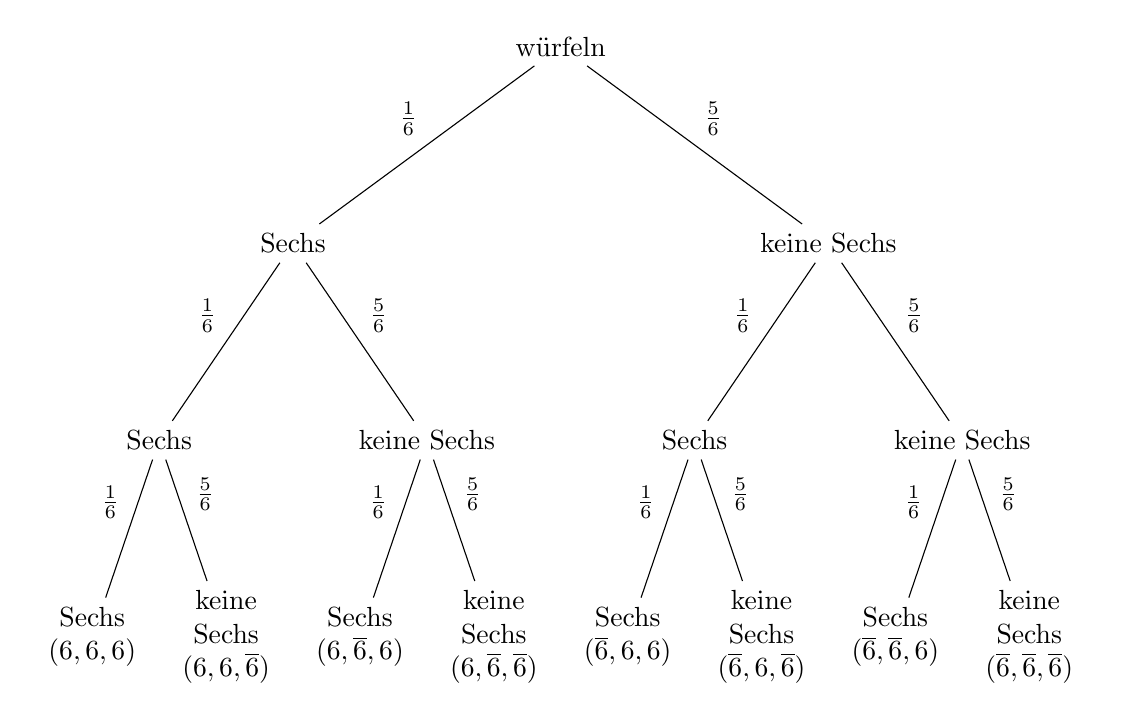
\begin{tikzpicture}[grow=down]
    \tikzstyle{level 1} = [level distance=2.5cm, sibling distance=6.8cm]
    \tikzstyle{level 2} = [level distance=2.5cm, sibling distance=3.4cm]
    \tikzstyle{level 3} = [level distance=2.5cm, sibling distance=1.7cm]
    \tikzstyle{leaf} = [text width=4em, text centered]
    \node {würfeln}
      child {
        node {Sechs}
        child {
          node {Sechs}
          child {
            node[leaf] {Sechs $(6, 6, 6)$}
            edge from parent
            node[above left] {$\frac{1}{6}$}
          }
          child {
            node[leaf] {keine Sechs $(6, 6, \overline{6})$}
            edge from parent
            node[above right] {$\frac{5}{6}$}
          }
          edge from parent
          node[above left] {$\frac{1}{6}$}
        }
        child {
          node {keine Sechs}
          child {
            node[leaf] {Sechs $(6, \overline{6}, 6)$}
            edge from parent
            node[above left] {$\frac{1}{6}$}
          }
          child {
            node[leaf] {keine Sechs $(6, \overline{6}, \overline{6})$}
            edge from parent
            node[above right] {$\frac{5}{6}$}
          }
          edge from parent
          node[above right] {$\frac{5}{6}$}
        }
        edge from parent
        node[above left] {$\frac{1}{6}$}
      }
      child {
        node {keine Sechs}
        child {
          node {Sechs}
          child {
            node[leaf] {Sechs $(\overline{6}, 6, 6)$}
            edge from parent
            node[above left] {$\frac{1}{6}$}
          }
          child {
            node[leaf] {keine Sechs $(\overline{6}, 6, \overline{6})$}
            edge from parent
            node[above right] {$\frac{5}{6}$}
          }
          edge from parent
          node[above left] {$\frac{1}{6}$}
        }
        child {
          node {keine Sechs}
          child {
            node[leaf] {Sechs $(\overline{6}, \overline{6}, 6)$}
            edge from parent
            node[above left] {$\frac{1}{6}$}
          }
          child {
            node[leaf] {keine Sechs $(\overline{6}, \overline{6}, \overline{6})$}
            edge from parent
            node[above right] {$\frac{5}{6}$}
          }
          edge from parent
          node[above right] {$\frac{5}{6}$}
        }
        edge from parent
        node[above right] {$\frac{5}{6}$}
      };
    \end{tikzpicture}
\end{gather*}
\begin{gather*}
  S = \{(6, 6, 6), (6, 6, \overline{6}), ...\} \quad \text{(Ergebnismenge)} \\
  |S| = 2^3 = 8
\end{gather*}
Jeder Pfad führt zu einem Ergebnis $e$ \\
Jeder Pfad besteht hier aus $3$ Zweigen (dreistufig) \\\\
Die Pfadwahrscheinlichkeit ist das Produkt der Zweige $w$ entlang des Pfades, \\
z. B. $P((6, \overline{6}, \overline{6})) = \frac{1}{6} \cdot \frac{5}{6} \cdot \frac{5}{6} = \frac{25}{216}$ \\\\
$E_1$: genau zwei Sechsen bei drei Würfen \\
Ereignis $E_1$ besteht aus drei Ergebnissen ($(6, 6, \overline{6})$, $(6, \overline{6}, 6)$, $(\overline{6}, 6, 6)$) \\
Die Wahrscheinlichkeit von $E_1$ ist die Summe der Wahrscheinlichkeiten der Ergebnisse
$P(E_1) = \frac{1}{6} \cdot \frac{1}{6} \cdot \frac{5}{6} + \frac{1}{6} \cdot \frac{5}{6} \cdot \frac{1}{6} + \frac{5}{6} \cdot \frac{1}{6} \cdot \frac{1}{6} = \frac{15}{216} = \frac{5}{72}$ \\
\textbf{Beispiel: 3 Züge ohne Zurücklegen (anfangs $2$ rote, $3$ gelbe Kugeln)}
\begin{gather*}
  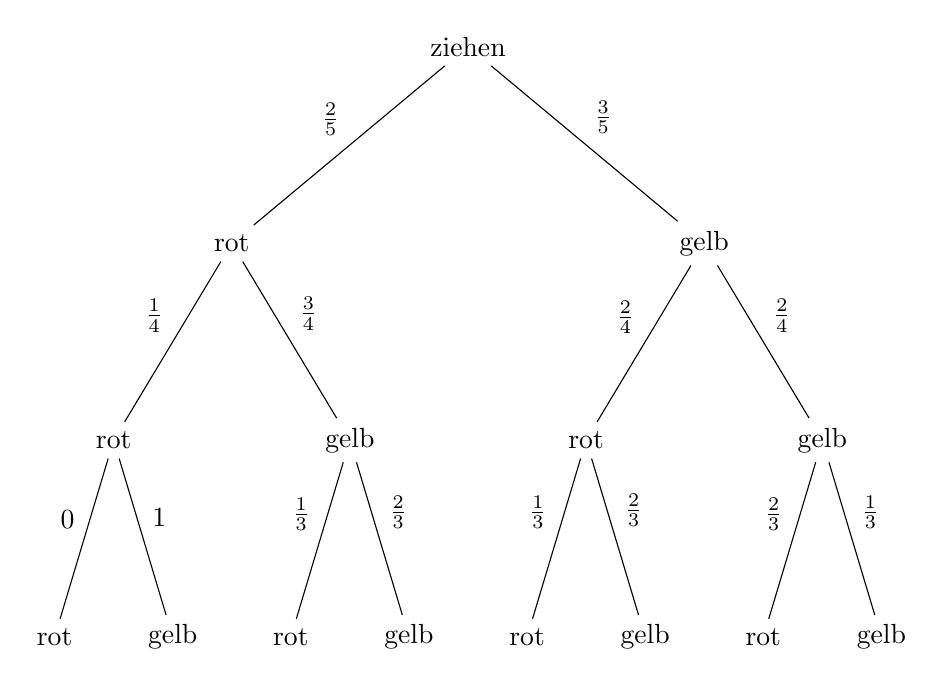
\begin{tikzpicture}[grow=down]
    \tikzstyle{level 1} = [level distance=2.5cm, sibling distance=6cm]
    \tikzstyle{level 2} = [level distance=2.5cm, sibling distance=3cm]
    \tikzstyle{level 3} = [level distance=2.5cm, sibling distance=1.5cm]
    \node {ziehen}
      child {
        node {rot}
        child {
          node {rot}
          child {
            node {rot}
            edge from parent
            node[above left] {$0$}
          }
          child {
            node {gelb}
            edge from parent
            node[above right] {$1$}
          }
          edge from parent
          node[above left] {$\frac{1}{4}$}
        }
        child {
          node {gelb}
          child {
            node {rot}
            edge from parent
            node[above left] {$\frac{1}{3}$}
          }
          child {
            node {gelb}
            edge from parent
            node[above right] {$\frac{2}{3}$}
          }
          edge from parent
          node[above right] {$\frac{3}{4}$}
        }
        edge from parent
        node[above left] {$\frac{2}{5}$}
      }
      child {
        node {gelb}
        child {
          node {rot}
          child {
            node {rot}
            edge from parent
            node[above left] {$\frac{1}{3}$}
          }
          child {
            node {gelb}
            edge from parent
            node[above right] {$\frac{2}{3}$}
          }
          edge from parent
          node[above left] {$\frac{2}{4}$}
        }
        child {
          node {gelb}
          child {
            node {rot}
            edge from parent
            node[above left] {$\frac{2}{3}$}
          }
          child {
            node {gelb}
            edge from parent
            node[above right] {$\frac{1}{3}$}
          }
          edge from parent
          node[above right] {$\frac{2}{4}$}
        }
        edge from parent
        node[above right] {$\frac{3}{5}$}
      };
    \end{tikzpicture}
\end{gather*}
\begin{exercise}{455/1}
  \item [a]
  \begin{gather*}
    \text{m. Z.} \quad P((r, r)) = \frac{4}{7} \cdot \frac{4}{7} = \frac{16}{49} \\
    \text{o. Z.} \quad P((r, r)) = \frac{4}{7} \cdot \frac{3}{6} = \frac{2}{7}
  \end{gather*}
  \item [b]
  \begin{gather*}
    \text{m. Z.} \quad P((r, b)) = 2 \cdot \frac{4}{7} \cdot \frac{3}{7} = \frac{24}{49} \\
    \text{o. Z.} \quad P((r, b)) = \frac{4}{7} \cdot \frac{3}{6} + \frac{3}{7} \cdot \frac{4}{6} = \frac{4}{7}
  \end{gather*}
  \item [c]
  \begin{gather*}
    \text{m. Z.} \quad P((r, r), (r, b)) = \frac{16}{49} + \frac{24}{49} = \frac{40}{49} \\
    \text{o. Z.} \quad P((r, r), (r, b)) = \frac{2}{7} + \frac{4}{7} = \frac{6}{7}
  \end{gather*}
  \item [d]
  \begin{gather*}
    \text{m. Z.} \quad P((r, r), (r, b)) = \frac{40}{49} \\
    \text{o. Z.} \quad P((r, r), (r, b)) = \frac{6}{7}
  \end{gather*}
\end{exercise}
